\documentclass[fleqn,10pt]{wlscirep}
\usepackage[utf8]{inputenc}
\usepackage[T1]{fontenc}
\usepackage{lineno}
\usepackage{array}
\usepackage{multirow}
\usepackage{float}
\linenumbers

\title{Multi-Domain Deepfake Detection via Decoupled Spatial-Frequency Feature Learning and Sample-Dependent Multi-Token Attention Fusion}

\author[1,*]{Abdelrahman Hassan}
\author[1]{Ahmed Hassan}
\author[1]{Hossam Abdelmunim}
\affil[1]{Computer and Systems Engineering Department, Faculty of Engineering, Ain Shams University, Cairo, Egypt}
\affil[*]{2201662@eng.asu.edu.eg}

\begin{abstract}
Detecting synthetic facial imagery across heterogeneous generative models remains challenging because spatial-domain and frequency-domain detectors exhibit complementary strengths and failure modes. This study presents a decoupled two-stage multi-domain deepfake detection framework combining a spatial RGB ResNet-50 expert (\texttt{Wang2020\_128}, 23.77M parameters) and a lightweight three-level Haar wavelet-packet convolutional expert (\texttt{Wolter2021\_128}, 1.73M parameters, 192 spectral sub-bands), each projecting to a supervised 128-dimensional embedding before freezing. Addressing the single-token attention degeneracy where sequence length $T=1$ collapses softmax weights to unity, we replace single-token cross-attention with genuinely sample-dependent multi-token self-attention (\texttt{MHA\_128}, 199,425 parameters over $[\mathbf{x}_{\text{cls}}, \mathbf{x}_s, \mathbf{x}_f]$) alongside a lightweight modality-gating module (\texttt{GatedFusion}, 41,987 parameters) and three capacity-matched controls ($\approx$198K--199K parameters). To prevent base-expert memorization bias and format shortcuts, experts are trained on 439,222 images spanning four native high-resolution authentic face sources and thirteen diffusion generators under a Leave-One-Generator-Out (LOGO) split, while fusion heads are cross-fitted on 58,103 out-of-sample held-out images and evaluated on untouched in-domain ($n=12,729$) and four unseen photorealistic domains (LFW camera reals vs.\ unseen LDM, SDXL\_Refine, DiffFace, and StyleGAN) under matched JPEG $Q=85$ recompression. Across four seeds, cross-fitted fusion lifts held-out accuracy from 98.76\% (RGB) and 97.53\% (Wavelet) to 99.12\% (\texttt{MHA\_128}, 0.9997 ROC-AUC, 0.87\% EER) and ranks first on strictly native PNG-only controls (98.90\%, 0.9996 AUC), while decisively outperforming unfrozen joint end-to-end training (52.10\% unseen accuracy, 4.5\% real recall). Under unseen domain shift, \texttt{MHA\_128} achieves the lowest probability calibration error ($\text{ECE}=0.039$), whereas lightweight \texttt{GatedFusion} achieves the highest four-domain unseen mean accuracy ($85.71\% \pm 0.06\%$, $0.9164$ AUC) and perturbation resilience (97.7\% at JPEG $Q=30$), while fair-attribute auditing on held-out FairFace validation faces yields $0.00\%$ false-positive disparity across race, gender, and age.
\end{abstract}

\begin{document}

\flushbottom
\maketitle
\thispagestyle{empty}

\noindent\textbf{Keywords:} deepfake detection, frequency-domain forensics, wavelet packet decomposition, spatial-frequency fusion, multi-head attention, cross-domain generalization.

\section*{Introduction}

\subsection*{Problem Context and Forensic Motivation}
Modern generative models---spanning Generative Adversarial Networks (GANs), pixel-space denoising diffusion models (ADM, DDPM, DDIM) \cite{ref1,ref2,ref3}, latent diffusion architectures (LDM, SDXL), and diffusion-based face swapping (DiffSwap, DiffFace) \cite{ref16,ref21}---synthesize photorealistic facial media that routinely deceive human observers. Although visually convincing, each synthesis paradigm introduces subtle statistical regularities during spatial upsampling, local boundary blending, or iterative denoising \cite{ref4,ref5}. Single-modality detectors often trade off sensitivity against specificity when deployed across heterogeneous generation pipelines and post-processing degradations.

\subsection*{Spatial-Frequency Trade-Offs and Motivation for Sample-Dependent Fusion}
Spatial convolutional backbones operating on RGB pixels effectively capture localized semantic artifacts and face-swap seams \cite{ref4,ref28}, yet end-to-end fine-tuned CNNs can over-specialize to seen training generators and exhibit elevated false-positive rates on out-of-distribution camera imagery \cite{ref5,ref31}. Conversely, frequency-domain wavelet-packet networks isolate multi-scale spectral anomalies across approximation and detail sub-bands \cite{ref8} and exhibit strong resilience to compression, yet lack high-level semantic context.

Combining spatial and frequency cues via static feature concatenation applies fixed global weights identically to every image, regardless of compression severity or conflicting modality reliability. Furthermore, our prior single-token cross-attention formulation ($T=1$) mathematically collapsed attention weights to $\text{Softmax}(s)=1.0$ identically for all inputs, preventing true sample-dependent weighting. In this revised work, we directly resolve that theoretical contradiction by introducing genuinely sample-dependent multi-token self-attention (\texttt{MHA\_128} over a three-token sequence $[\mathbf{x}_{\text{cls}}, \mathbf{x}_s, \mathbf{x}_f]$) and explicit sample-dependent modality gating (\texttt{GatedFusion}), and by benchmarking both against strictly capacity-matched ($\approx$199K-parameter) pure-MLP, FFN-only, and linear-mixing controls under an out-of-sample cross-fitted protocol.

Specifically, our contributions are:
\begin{enumerate}
    \item \textbf{Clarified Modular Two-Stage Architecture with Exact Parameter Accounting:} We adapt two established domain experts---\texttt{Wang2020\_128} (ResNet-50 \cite{ref4} augmented with a supervised 128-D bottleneck; 23,770,433 parameters) and \texttt{Wolter2021\_128} (3-level Haar Wavelet Packet CNN \cite{ref8} with 192 spectral sub-bands and a 128-D bottleneck; 1,727,553 parameters)---and empirically demonstrate via a controlled unfrozen joint-training baseline that staged decoupling prevents severe unseen-real collapse (4.5\% vs.\ 90.3\%--94.8\% unseen real recall).
    \item \textbf{True Sample-Dependent Multi-Token Attention \& Capacity-Matched Ablation Suite:} We replace degenerate single-token attention with three-token multi-head self-attention (\texttt{MHA\_128}, 199,425 parameters) and sample-dependent \texttt{GatedFusion} (41,987 parameters), and rigorously isolate attention vs.\ feed-forward capacity against three 1:1 parameter-matched controls (\texttt{ConcatMatchedMLP}, \texttt{NoAttnFFN}, \texttt{LinearMix}) across $N=4$ independent seeds with Holm--Bonferroni multiplicity correction, probability calibration metrics (Brier score, ECE, reliability diagrams), and a 16-configuration concatenation width/dropout sweep.
    \item \textbf{Shortcut-Free Multi-Domain Benchmark, Cross-Fitted Stacking, and Comprehensive Audits:} We construct a verified 556,082-image multi-domain benchmark combining four native high-resolution authentic face datasets (FairFace, CelebA, FFHQ-256, UTKFace) and fifteen balanced diffusion/face-swap generators under a Leave-One-Generator-Out (LOGO) split, enforce out-of-sample cross-fitted fusion training to eliminate base-expert memorization bias, and report per-generator recall/AUC, strictly native PNG-only same-pipeline controls, matched JPEG $Q=85$ unseen cross-domain generalization (LFW vs.\ LDM, SDXL\_Refine, DiffFace, StyleGAN), end-to-end raw-pixel white-box FGSM sweeps, nine real-world perturbations, and FairFace ground-truth demographic fairness audits.
\end{enumerate}

\section*{Related Work}

\subsection*{Spatial-Domain and Universal Foundation Detectors}
Early spatial forgery detectors relied on compact or depthwise-separable CNNs such as MesoNet \cite{ref24} and Xception \cite{ref28}. Wang et al.\ \cite{ref4} established that ResNet-50 trained with aggressive Gaussian blur and JPEG compression augmentations generalizes across multiple CNN generators, while Ricker et al.\ \cite{ref5} analyzed spatial artifacts of denoising diffusion models (ADM, DDPM, DDIM). Subsequent spatial approaches targeted forgery-invariant feature disentanglement, including UCF \cite{ref31}, semantic decoupling \cite{ref29}, and convolutional vision-transformer hybrids \cite{ref30}. More recently, universal detectors leveraging frozen vision-language foundation models (e.g., CLIP feature space \cite{ref41}) and diffusion reconstruction contrastive learning (DRCT \cite{ref42}) have demonstrated strong transfer across unseen generative families, highlighting the limitations of end-to-end fine-tuned CNN backbones under severe paradigm shift. In this study, we focus specifically on controlled spatial--frequency fusion over fixed CNN and wavelet experts without claiming global state-of-the-art superiority over large foundation-model detectors.

\subsection*{Frequency-Domain and Spatial-Frequency Fusion Forensics}
Frequency-domain detectors analyze spectral irregularities via Fourier transforms, DCT coefficients, or multi-scale wavelets. Wolter et al.\ \cite{ref8} introduced full Wavelet Packet Decomposition (WPD) CNNs that preserve spatial-frequency localization across recursive sub-bands, while earlier dual-stream fusion architectures combined RGB and spectral cues through dual-attention or information decomposition \cite{ref6,ref7}. Recent spatial-frequency works have advanced dual-domain integration substantially: FreqDebias (CVPR 2025) \cite{ref45} mitigates spectral shortcut bias via consistency-driven frequency debiasing; FAViT (2026) \cite{ref43} combines a frequency-aware Vision Transformer with bidirectional cross-attention for post-processing robustness; and LGF-Net (2026) \cite{ref44} integrates learnable Gabor filters with gated cross-modal fusion. Unlike monolithic end-to-end dual-branch architectures, our work isolates the fusion mechanism under strictly frozen 128-D experts, cross-fitted out-of-sample stacking, and 1:1 parameter-matched structural ablations so that performance differences can be attributed transparently to sample-dependent weighting, capacity, or modality complementarity rather than confounded backbone updates.

\section*{Proposed Multi-Domain Detection Framework}

\subsection*{Attribution of Adopted vs.\ Newly Introduced Components}
To make architectural increments transparent (overview in Figure~\ref{fig:architecture}), we explicitly distinguish adopted baselines from components newly introduced in this study:
\begin{itemize}
    \item \textbf{Adopted Backbones:} The ResNet-50 convolutional trunk from Wang et al.\ \cite{ref4,ref25} (23,508,032 parameters) and the 4-block Wavelet Packet CNN trunk from Wolter et al.\ \cite{ref8} (1,661,760 parameters over 3-level Haar packets).
    \item \textbf{New Contributions in This Study:} (i) Supervised 128-D latent projection bottlenecks appended to both experts; (ii) GPU-batched differentiable 3-level Haar WPD with $\text{signed\_log1p}$ scaling; (iii) sample-dependent three-token multi-head self-attention (\texttt{MHA\_128}, 199,425 parameters) and modality gating (\texttt{GatedFusion}, 41,987 parameters); (iv) exact capacity-matched structural ablation heads (\texttt{ConcatMatchedMLP}, \texttt{NoAttnFFN}, \texttt{LinearMix}); and (v) an out-of-sample cross-fitted staged training protocol eliminating base-expert memorization bias.
\end{itemize}

\begin{figure}[tbp]
\centering
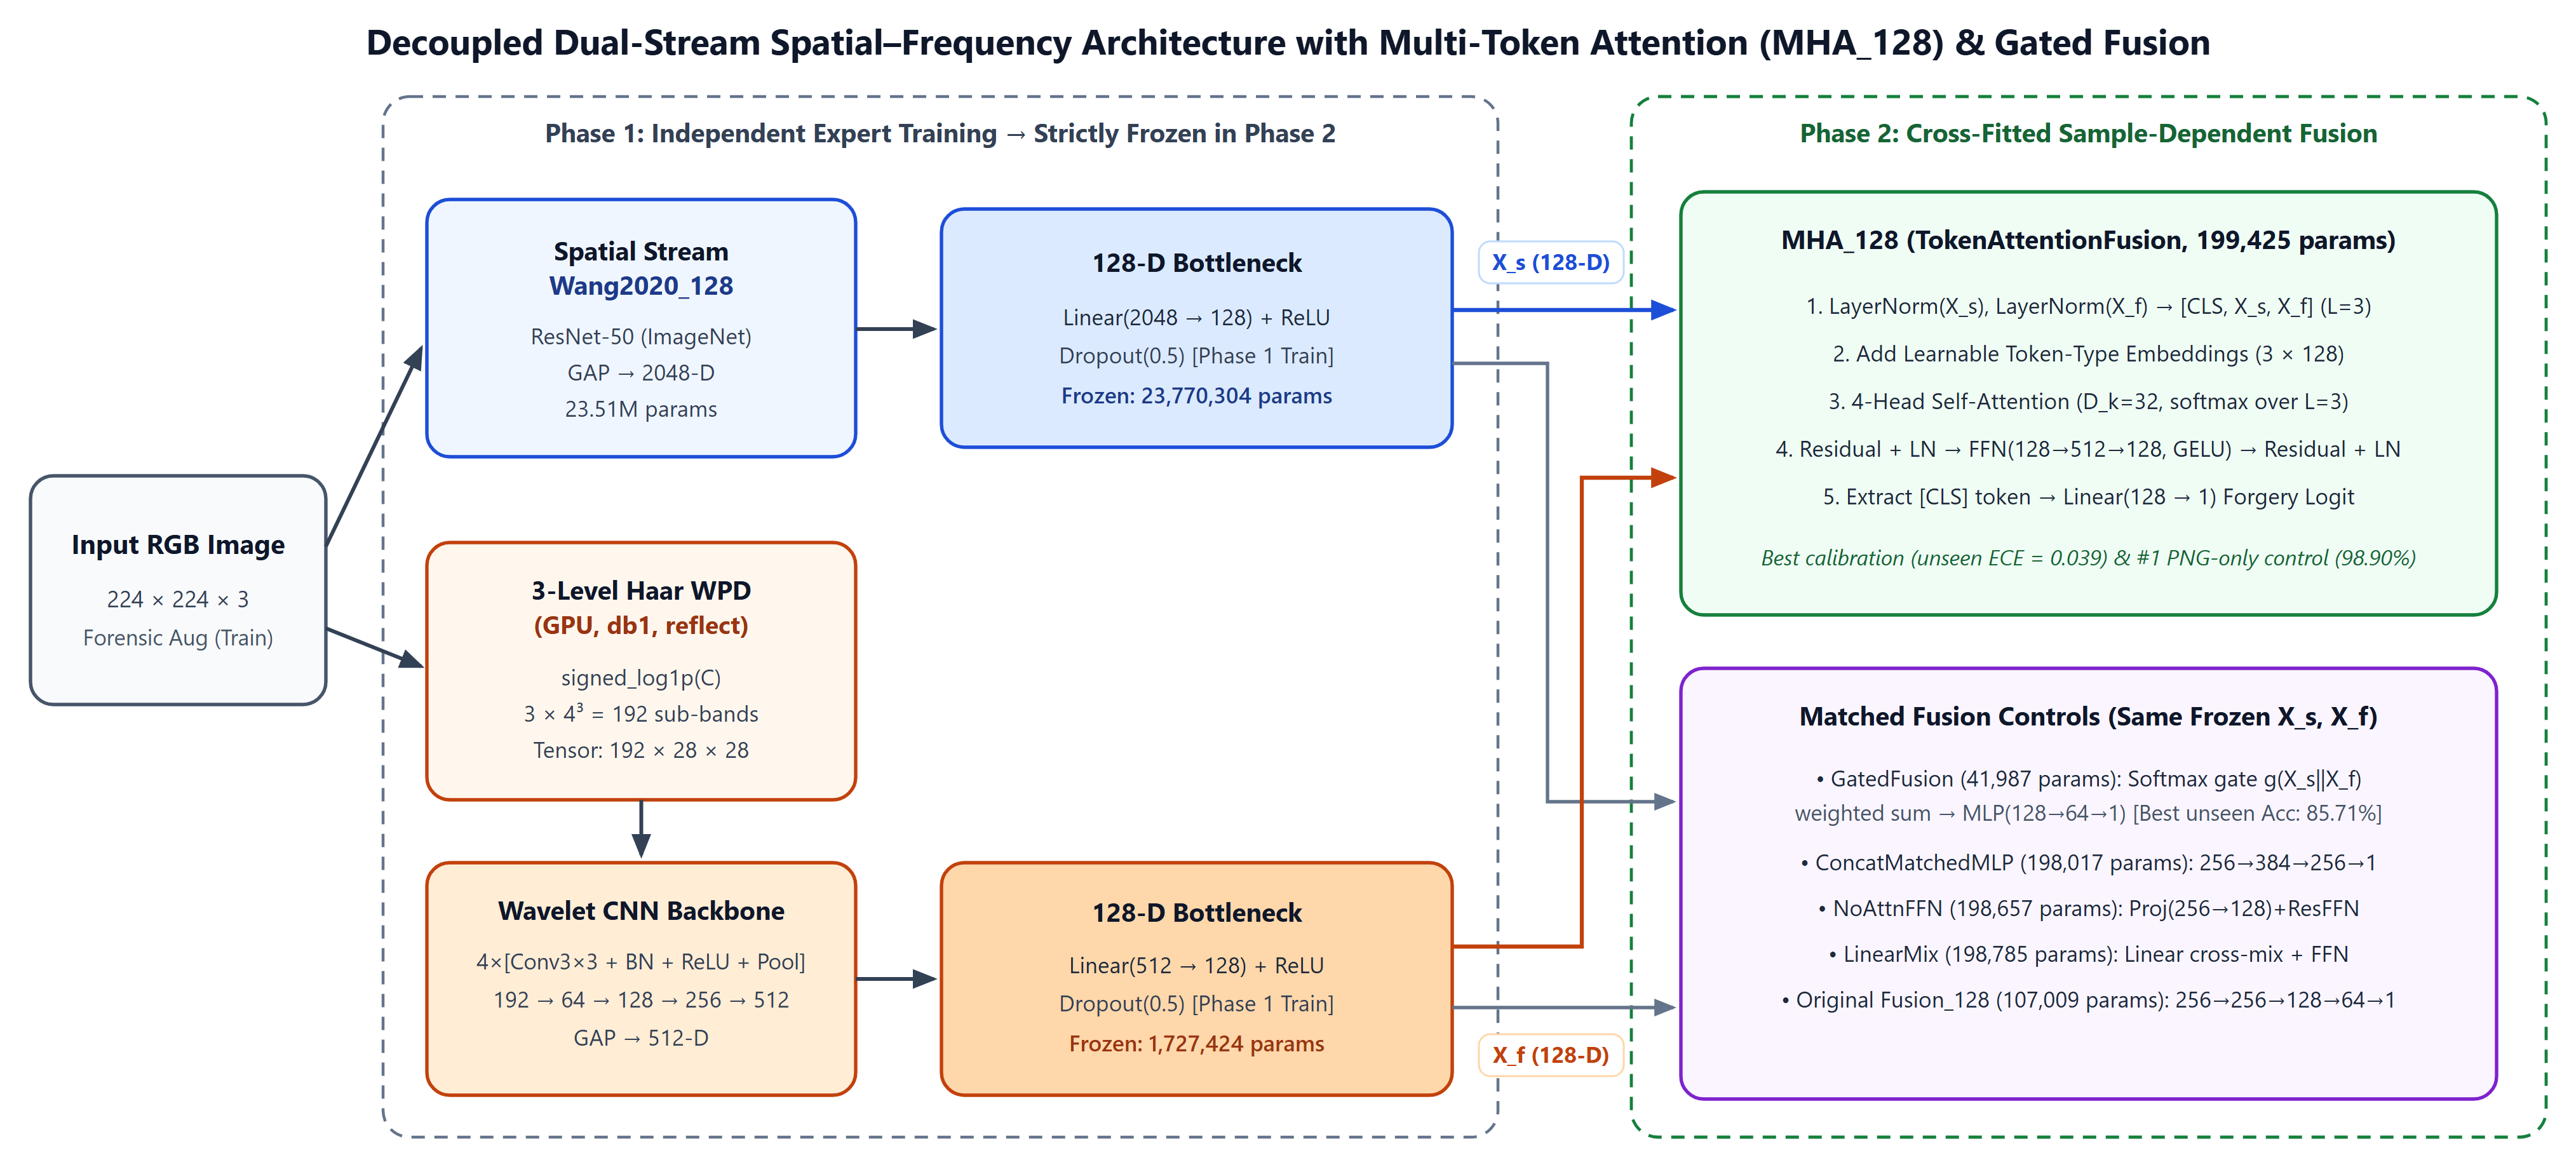
\includegraphics[width=\linewidth]{figures/fig1_architecture.png}
\caption{Complete decoupled dual-stream architecture showing exact tensor dimensions, layer sequences, and trainable parameter counts across Phase 1 (independent spatial \texttt{Wang2020\_128} and frequency \texttt{Wolter2021\_128} experts) and Phase 2 (cross-fitted sample-dependent \texttt{MHA\_128} multi-token self-attention and matched fusion controls).}
\label{fig:architecture}
\end{figure}

\subsection*{Phase 1: Spatial and Frequency Experts with 128-D Bottlenecks}
\paragraph{Spatial Expert (\texttt{Wang2020\_128}).}
An input RGB image resized to $224 \times 224 \times 3$ and ImageNet-normalized is encoded by ResNet-50 into a global-average-pooled descriptor $\mathbf{h}_s \in \mathbb{R}^{2048}$. A supervised bottleneck maps $\mathbf{h}_s$ to $\mathbf{x}_s \in \mathbb{R}^{128}$:
\begin{equation}
\mathbf{x}_s = \operatorname{ReLU}\!\left(\mathbf{W}_{s,\text{proj}}\mathbf{h}_s + \mathbf{b}_{s,\text{proj}}\right) \in \mathbb{R}^{128},
\label{eq:spatial_embed}
\end{equation}
where $\mathbf{W}_{s,\text{proj}} \in \mathbb{R}^{128 \times 2048}$ and $\mathbf{b}_{s,\text{proj}} \in \mathbb{R}^{128}$. During Phase 1 training, $\operatorname{Dropout}(0.5)$ and a linear classifier $\mathbf{w}_s^\top \mathbf{x}_s + b_s$ are applied under label-smoothed binary cross-entropy ($s=0.05$). After convergence, the 129-parameter temporary linear head is discarded and all 23,770,304 remaining backbone and bottleneck parameters are frozen in evaluation mode.

\paragraph{Frequency Expert (\texttt{Wolter2021\_128}).}
Each $224 \times 224$ RGB channel (in $[0,255]$ float32) undergoes a three-level 2D orthogonal Haar (\texttt{db1}) Wavelet Packet Decomposition with reflection padding on GPU, yielding $3 \times 4^3 = 192$ spectral sub-bands of spatial size $28 \times 28$ (tensor shape $192 \times 28 \times 28$). To compress heavy-tailed magnitudes while preserving coefficient polarity, we apply signed logarithmic scaling:
\begin{equation}
\tilde{C}_{c,u,v} = \operatorname{sign}\!\left(C_{c,u,v}\right)\log\!\left(1 + \lvert C_{c,u,v} \rvert\right).
\label{eq:wavelet_log}
\end{equation}
The $192 \times 28 \times 28$ tensor is processed by four sequential convolutional blocks---$\text{Conv}_{3\times 3}(\text{pad}=1) \to \text{BatchNorm2d} \to \text{ReLU} \to \text{MaxPool}_{2\times 2}$---with exact channel progression $192 \to 64 \to 128 \to 256 \to 512$ (spatial maps $28\times 28 \to 14\times 14 \to 7\times 7 \to 3\times 3 \to 1\times 1$), followed by global average pooling to $\mathbf{h}_f \in \mathbb{R}^{512}$ and the 128-D bottleneck:
\begin{equation}
\mathbf{x}_f = \operatorname{ReLU}\!\left(\mathbf{W}_{f,\text{proj}}\mathbf{h}_f + \mathbf{b}_{f,\text{proj}}\right) \in \mathbb{R}^{128},
\label{eq:freq_embed}
\end{equation}
where $\mathbf{W}_{f,\text{proj}} \in \mathbb{R}^{128 \times 512}$ and $\mathbf{b}_{f,\text{proj}} \in \mathbb{R}^{128}$. Including the Phase 1 temporary linear head ($128 \to 1$), the exact parameter count is $1,727,553$ (Table~\ref{tab:arch_params}).

\subsection*{Phase 2: Sample-Dependent Multi-Token Attention (\texttt{MHA\_128}) and Matched Controls}
\paragraph{Resolving Single-Token Softmax Degeneracy.}
When scaled dot-product attention is applied to a single key token ($T=1$), $\operatorname{Softmax}\!\left(\mathbf{q}^\top\mathbf{k}/\sqrt{D_k}\right) = \exp(s)/\exp(s) = 1.0$ identically for every input sample, preventing competitive weighting across modalities. To achieve genuine sample-dependent weighting, \texttt{MHA\_128} (\texttt{TokenAttentionFusion}) constructs a three-token sequence $\mathbf{H}_0 \in \mathbb{R}^{3 \times D}$ ($D=128$, sequence length $L=3$) by prepending a learnable classification token $\mathbf{x}_{\text{cls}} \in \mathbb{R}^{1 \times D}$ to the layer-normalized spatial and frequency embeddings and adding learnable modality-type embeddings $\mathbf{E}_{\text{type}} \in \mathbb{R}^{3 \times D}$:
\begin{equation}
\mathbf{H}_0 = \begin{bmatrix} \mathbf{x}_{\text{cls}} \\ \operatorname{LN}_s(\mathbf{x}_s)^\top \\ \operatorname{LN}_f(\mathbf{x}_f)^\top \end{bmatrix} + \mathbf{E}_{\text{type}} \in \mathbb{R}^{3 \times 128}.
\label{eq:token_seq}
\end{equation}
Multi-head self-attention with $N_{\text{heads}}=4$ heads ($D_k = D/4 = 32$) computes per-head projections with explicit learnable biases:
\begin{equation}
\mathbf{Q}^{(h)} = \mathbf{H}_0 \mathbf{W}^{Q,(h)} + \mathbf{1}\mathbf{b}^{Q,(h)\top}, \quad
\mathbf{K}^{(h)} = \mathbf{H}_0 \mathbf{W}^{K,(h)} + \mathbf{1}\mathbf{b}^{K,(h)\top}, \quad
\mathbf{V}^{(h)} = \mathbf{H}_0 \mathbf{W}^{V,(h)} + \mathbf{1}\mathbf{b}^{V,(h)\top},
\label{eq:qkv}
\end{equation}
where $\mathbf{W}^{Q,(h)},\mathbf{W}^{K,(h)},\mathbf{W}^{V,(h)} \in \mathbb{R}^{128 \times 32}$ and $\mathbf{b}^{Q,(h)},\mathbf{b}^{K,(h)},\mathbf{b}^{V,(h)} \in \mathbb{R}^{32}$. Because each query attends over $L=3$ distinct keys ($\{\text{CLS}, \text{RGB}, \text{Wavelet}\}$), the attention weights $\boldsymbol{\alpha}^{(h)} = \operatorname{Softmax}\!\left(\mathbf{Q}^{(h)}(\mathbf{K}^{(h)})^\top/\sqrt{D_k}\right) \in \mathbb{R}^{3 \times 3}$ vary strictly as a function of each input image:
\begin{equation}
\operatorname{MHA}(\mathbf{H}_0) = \operatorname{Concat}\!\left(\boldsymbol{\alpha}^{(1)}\mathbf{V}^{(1)}, \dots, \boldsymbol{\alpha}^{(4)}\mathbf{V}^{(4)}\right)\mathbf{W}^O + \mathbf{1}\mathbf{b}^{O\top}.
\label{eq:mha_out}
\end{equation}
Standard pre-/post-residual Transformer blocks with LayerNorm and a GELU feed-forward network ($128 \to 512 \to 128$, dropout $p=0.2$) refine all three tokens, and the refined $[\text{CLS}]$ token produces the raw forgery logit $y \in \mathbb{R}$:
\begin{align}
\mathbf{H}_1 &= \operatorname{LN}_1\!\left(\mathbf{H}_0 + \operatorname{MHA}(\mathbf{H}_0)\right), \label{eq:res1}\\
\mathbf{H}_2 &= \operatorname{LN}_2\!\left(\mathbf{H}_1 + \operatorname{FFN}(\mathbf{H}_1)\right), \label{eq:res2}\\
\operatorname{FFN}(\mathbf{Z}) &= \operatorname{Drop}\!\left(\operatorname{Drop}\!\left(\operatorname{GELU}(\mathbf{Z}\mathbf{W}_1 + \mathbf{1}\mathbf{b}_1^\top)\right)\mathbf{W}_2 + \mathbf{1}\mathbf{b}_2^\top\right), \label{eq:ffn}\\
y &= \mathbf{w}_{\text{cls}}^\top \mathbf{H}_{2,\text{cls}}^\top + b_{\text{cls}}. \label{eq:logit}
\end{align}

\paragraph{Explicit Sample-Dependent Gating and Capacity-Matched Structural Controls.}
To strictly disentangle attention routing from parameter capacity and feed-forward refinement, we evaluate five controlled alternatives on the exact same frozen $(\mathbf{x}_s, \mathbf{x}_f)$ embeddings (Table~\ref{tab:arch_params}):
\begin{enumerate}
    \item \textbf{\texttt{GatedFusion} (41,987 params):} Computes sample-dependent softmax modality weights and gated sum
    \[\mathbf{g} = \operatorname{Softmax}\!\left(\operatorname{MLP}_{\text{gate}}\!\left([\operatorname{LN}_s(\mathbf{x}_s)\,\|\,\operatorname{LN}_f(\mathbf{x}_f)]\right)\right) \in \Delta^1, \qquad \mathbf{z} = g_s \operatorname{LN}_s(\mathbf{x}_s) + g_f \operatorname{LN}_f(\mathbf{x}_f),\]
    followed by a lightweight classifier $\text{MLP}(128 \to 64 \to 1)$.
    \item \textbf{\texttt{ConcatMatchedMLP} (198,017 params; $0.993\times$ of \texttt{MHA\_128}):} Pure-MLP concatenation control $\operatorname{LN}_s(\mathbf{x}_s)\|\operatorname{LN}_f(\mathbf{x}_f) \to 384 \to 256 \to 1$ with GELU and dropout.
    \item \textbf{\texttt{NoAttnFFN} (198,657 params; $0.996\times$):} Direct single-direction affine projection $\mathbf{z} = \mathbf{W}[\operatorname{LN}_s(\mathbf{x}_s)\,\|\,\operatorname{LN}_f(\mathbf{x}_f)] + \mathbf{b}$ ($\text{Linear}(256\to 128)$) followed by a capacity-matched residual FFN ($128 \to 640 \to 128$) without attention.
    \item \textbf{\texttt{LinearMix} (198,785 params; $0.997\times$):} Fixed linear cross-mixing ($\mathbf{r}_{\text{mix}} = \mathbf{r} + \mathbf{W}_w \mathbf{w}$, $\mathbf{w}_{\text{mix}} = \mathbf{w} + \mathbf{W}_r \mathbf{r}$) without softmax, projected $256 \to 128$ into an identical $128 \to 512 \to 128$ FFN.
    \item \textbf{\texttt{Fusion\_128} (107,009 params):} Original static concatenation MLP ($256 \to 256 \to 128 \to 64 \to 1$) retained for longitudinal continuity.
\end{enumerate}

\begin{table}[tbp]
\centering
\caption{Exact component-level and layer-by-layer parameter specifications (224$\times$224 input). Adopted trunks are explicitly separated from newly introduced bottleneck and fusion modules.}
\label{tab:arch_params}
\small
\begin{tabular}{@{}llrr@{}}
\toprule
\textbf{Module / Component} & \textbf{Exact Layer Specification} & \textbf{Output Shape} & \textbf{Parameters} \\
\midrule
\multicolumn{4}{@{}l}{\textit{Phase 1: Spatial Expert (\texttt{Wang2020\_128}) — Frozen in Phase 2}} \\
ResNet-50 Trunk (adopted \cite{ref4}) & Conv1 + Layers 1--4 + GlobalAvgPool & $1 \times 2048$ & 23,508,032 \\
128-D Bottleneck (new) & $\text{Linear}(2048\to 128) + \text{ReLU} + \text{Drop}(0.5)$ & $1 \times 128$ & 262,272 \\
Phase-1 Temp Head (discarded) & $\text{Linear}(128\to 1)$ & $1 \times 1$ & 129 \\
\textbf{Subtotal \texttt{Wang2020\_128}} & & & \textbf{23,770,433} \\
\midrule
\multicolumn{4}{@{}l}{\textit{Phase 1: Frequency Expert (\texttt{Wolter2021\_128}) — Frozen in Phase 2}} \\
3-Level Haar WPD (GPU, new) & \texttt{db1}, reflect pad, $\text{signed\_log1p}$ & $192 \times 28 \times 28$ & 0 \\
Conv Block 1 (adopted \cite{ref8}) & $\text{Conv}_{3\times 3}(192\to 64)+\text{BN}+\text{ReLU}+\text{Pool}_{2\times 2}$ & $64 \times 14 \times 14$ & 110,784 \\
Conv Block 2 (adopted \cite{ref8}) & $\text{Conv}_{3\times 3}(64\to 128)+\text{BN}+\text{ReLU}+\text{Pool}_{2\times 2}$ & $128 \times 7 \times 7$ & 74,112 \\
Conv Block 3 (adopted \cite{ref8}) & $\text{Conv}_{3\times 3}(128\to 256)+\text{BN}+\text{ReLU}+\text{Pool}_{2\times 2}$ & $256 \times 3 \times 3$ & 295,680 \\
Conv Block 4 + GAP (adopted \cite{ref8}) & $\text{Conv}_{3\times 3}(256\to 512)+\text{BN}+\text{ReLU}+\text{Pool}+\text{GAP}$ & $1 \times 512$ & 1,181,184 \\
128-D Bottleneck + Temp Head (new) & $\text{Linear}(512\to 128)+\text{ReLU}+\text{Drop}(0.5)+\text{Linear}(128\to 1)$ & $1 \times 128$ & 65,793 \\
\textbf{Subtotal \texttt{Wolter2021\_128}} & & & \textbf{1,727,553} \\
\midrule
\multicolumn{4}{@{}l}{\textit{Phase 2: Proposed \texttt{MHA\_128} (\texttt{TokenAttentionFusion}) — Trainable Core}} \\
Input Norms + Tokens & $\text{LN}_s(128), \text{LN}_f(128), \mathbf{x}_{\text{cls}}(1\times 128), \mathbf{E}_{\text{type}}(3\times 128)$ & $3 \times 128$ & 1,024 \\
4-Head Self-Attention & $N_{\text{heads}}=4, D_k=32, L=3$, bias=True & $3 \times 128$ & 66,048 \\
Residual LN1 + FFN + LN2 & $\text{LN}(128) + \text{Linear}(128\to 512\to 128, \text{GELU}) + \text{LN}(128)$ & $3 \times 128$ & 132,224 \\
Classification Head & Extract $[\text{CLS}] \to \text{Linear}(128\to 1)$ & $1 \times 1$ & 129 \\
\textbf{Total Trainable \texttt{MHA\_128}} & \textit{(Full dual-stream total: 25,697,153 excl.\ temp heads)} & & \textbf{199,425} \\
\midrule
\multicolumn{4}{@{}l}{\textit{Phase 2: Controlled Fusion Baselines (Exact Parameter Counts)}} \\
\texttt{ConcatMatchedMLP} & $\text{LN}_s\|\text{LN}_f \to 384 \to 256 \to 1$ (GELU, Drop 0.2) & $1 \times 1$ & 198,017 \\
\texttt{NoAttnFFN} & $\text{Proj}(256\to 128) + \text{ResFFN}(128\to 640\to 128) \to 1$ & $1 \times 1$ & 198,657 \\
\texttt{LinearMix} & Linear cross-mix $(128\to 128) + \text{FFN}(128\to 512\to 128) \to 1$ & $1 \times 1$ & 198,785 \\
\texttt{GatedFusion} & $\text{Gate}(256\to 128\to 2) + \text{MLP}(128\to 64\to 1)$ & $1 \times 1$ & 41,987 \\
\texttt{Fusion\_128} (Original) & $\text{Concat}(256) \to 256 \to 128 \to 64 \to 1$ & $1 \times 1$ & 107,009 \\
\bottomrule
\end{tabular}
\end{table}

\section*{Dataset Curation, Cross-Fitted Partitioning, and Forensic Preprocessing}

\subsection*{Eliminating Source-Pipeline Shortcuts (\texttt{DatasetMultiDomainClean\_v2})}
A critical audit of our earlier benchmark revealed that relying primarily on CelebA still JPEGs for the authentic class against PNG diffusion outputs creates low-level resolution and compression shortcuts. To eliminate acquisition shortcuts and expand coverage to modern latent-diffusion architectures, we curated \texttt{DatasetMultiDomainClean\_v2} (detailed in Table~\ref{tab:contingency}) comprising \textbf{556,082 verified intact facial images} (all verified via \texttt{PIL.Image.load()}, center-square-cropped, and bicubically standardized to $256\times 256$):
\begin{itemize}
    \item \textbf{Authentic Class (278,041 images across 4 native high-resolution datasets):} FairFace \cite{ref46} (86,744 train PNG + 9,430 val PNG), CelebA \cite{ref36} (80,000 train JPG + 20,000 val JPG), FFHQ-256 \cite{ref47} (56,000 train PNG + 14,000 val PNG), and UTKFace \cite{ref48} (11,867 train PNG). In training, 65.9\% of authentic images are native PNGs and 34.1\% are JPEGs, eliminating binary codec separation.
    \item \textbf{Synthetic Class (278,041 images across 15 generators):} Four pixel-diffusion/swap repositories from Zenodo \cite{ref9,ref10} (ADM \cite{ref3}, DDPM \cite{ref1}, DDIM \cite{ref2}, DiffSwap \cite{ref16}; 20,000 train / 5,000 val each) plus eleven extended editing, face-swapping, image-to-image, and text-to-image diffusion generators (CoDiff, cycle\_diff, DCFace, DiffFace \cite{ref21}, DreamBooth, FreeDoM\_I, FreeDoM\_T, HPS, LoRA, SDXL, SDXL\_Refine; capped at 15,000 train / 2,500 val each via identity-stratified sampling). Global cross-generator identity disjointness and zero overlap with external test sets were verified programmatically (\texttt{fake\_identity\_overlap = 0}, \texttt{real\_identity\_overlap = 0}).
\end{itemize}

\begin{table}[tbp]
\centering
\caption{Complete source-by-class contingency table for \texttt{DatasetMultiDomainClean\_v2} (556,082 verified images total: 278,041 Authentic + 278,041 Synthetic) and external completely unseen evaluation benchmarks. *The 30,000 training images from the two LOGO-held-out generators (\texttt{SDXL\_Refine}: 15,000; \texttt{DiffFace}: 15,000) are quarantined from Phase 1 and Phase 2 training, leaving $234,611 + 204,611 = 439,222$ active training images ($526,082$ active train+val images $+ 30,000$ quarantined LOGO train images $= 556,082$).}
\label{tab:contingency}
\small
\begin{tabular}{@{}lllrrr@{}}
\toprule
\textbf{Class} & \textbf{Source / Generator} & \textbf{Format} & \textbf{Train Pool} & \textbf{Val Pool} & \textbf{Role in Protocol} \\
\midrule
Authentic (0) & FairFace \cite{ref46} & PNG & 86,744 & 9,430 & Phase 1 Train / Phase 2--3 Val \\
Authentic (0) & CelebA \cite{ref36} & JPG & 80,000 & 20,000 & Phase 1 Train / Phase 2--3 Val \\
Authentic (0) & FFHQ-256 \cite{ref47} & PNG & 56,000 & 14,000 & Phase 1 Train / Phase 2--3 Val \\
Authentic (0) & UTKFace \cite{ref48} & PNG & 11,867 & 0 & Phase 1 Train only \\
\textbf{Total Authentic} & \textbf{4 sources} & \textbf{66\% PNG / 34\% JPG} & \textbf{234,611} & \textbf{43,430} & \textbf{278,041 total (50.0\%)} \\
\midrule
Synthetic (1) & ADM, DDPM, DDIM, DiffSwap (4$\times$20K/5K) & PNG & 80,000 & 20,000 & Seen (Phase 1--3) \\
Synthetic (1) & CoDiff, cycle\_diff, DCFace, DreamBooth, HPS, SDXL (6$\times$15K/2.5K) & PNG & 90,000 & 15,000 & Seen (Phase 1--3) \\
Synthetic (1) & FreeDoM\_I (12,434/1,718), FreeDoM\_T (13,776/1,912), LoRA (8,401/1,148) & PNG & 34,611 & 4,778 & Seen (Phase 1--3) \\
Synthetic (1) & \textbf{SDXL\_Refine} (I2I Latent Diffusion; 15K train quarantined) & PNG & \textit{0 (excl.)} & 2,500 & \textbf{LOGO Unseen Test} \\
Synthetic (1) & \textbf{DiffFace} \cite{ref21} (Diffusion Face Swap; 15K train quarantined) & PNG & \textit{0 (excl.)} & 1,152 & \textbf{LOGO Unseen Test} \\
\textbf{Total Synthetic} & \textbf{15 generators (13 seen + 2 LOGO)} & \textbf{100\% PNG} & \textbf{204,611*} & \textbf{43,430} & \textit{*excl.\ 30,000 LOGO train} \\
\midrule
\multicolumn{6}{@{}l}{\textit{Completely Untouched External Cross-Domain Benchmarks (Zero Images in Phase 1 or Phase 2)}} \\
Authentic (0) & LFW \cite{ref49} (Real-world camera photographs) & JPG & 0 & 1,000 & Unseen Real Reference \\
Synthetic (1) & Unseen LDM (Latent Diffusion) & PNG & 0 & 1,000 & Unseen External Diffusion \\
Synthetic (1) & Unseen StyleGAN (140k Real-and-Fake Faces; \textbf{0 GANs in train}) & JPG & 0 & 1,000 & Extreme Cross-Paradigm Test \\
\bottomrule
\end{tabular}
\end{table}

\subsection*{Strict Three-Way Cross-Fitted Staged Protocol and Forensic Augmentation}
To eliminate both validation-selection optimism and producer--consumer overfitting (where a fusion head trained on Phase 1 training embeddings sees memorized expert predictions rather than true out-of-sample error distributions), we enforce strict partition isolation across three stages. All dataset-provided aligned facial crops are resized directly via bilinear interpolation to $224 \times 224$ without external face re-detection or additional cropping:
\begin{enumerate}
    \item \textbf{Phase 1 (Base Experts):} \texttt{Wang2020\_128} (AdamW, $\text{lr}=2\times 10^{-4}$, weight decay $10^{-2}$, 5-epoch cosine schedule with best held-out validation checkpoint selected at epoch 1, label smoothing $s=0.05$, batch size 128, BF16 AMP on NVIDIA L4) and \texttt{Wolter2021\_128} (Adam, $\text{lr}=5\times 10^{-4}$, weight decay $10^{-4}$, 5-epoch cosine schedule, batch size 128) are trained independently on the 439,222 active LOGO training images (234,611 real + 204,611 fake across 13 seen generators) with symmetric forensic augmentations applied equally to both classes: dynamic JPEG compression ($p=0.8$, $Q\in\{50,60,70,75,80,85,90,95\}$, OpenCV/Pillow), Gaussian blur ($p=0.35$, $\sigma\in[0.1,2.0]$), and bilinear downscale-upscale resampling ($p=0.35$, scale $\in[0.55,1.0]$).
    \item \textbf{Phase 2 (Out-of-Sample Cross-Fitted Fusion Training):} Using the 83,208 seen-validation images that \textbf{neither expert ever trained on} (excluding LOGO generators \texttt{SDXL\_Refine} and \texttt{DiffFace}), we perform an identity-grouped stratified 70\% / 15\% / 15\% split into \texttt{fusion\_train} ($n=58,103$: 30,401 real across CelebA/FairFace/FFHQ + 27,702 fake across all 13 seen generators), \texttt{fusion\_dev} ($n=12,376$: strictly for checkpoint selection), and untouched \texttt{seen\_test} ($n=12,729$). Fusion heads are trained for 25 epochs (AdamW, $\text{lr}=3\times 10^{-4}$, weight decay $10^{-3}$, cosine schedule, label smoothing $s=0.05$, modality dropout $p=0.15$) on clean plus forensic-augmented views of \texttt{fusion\_train} across four independent seeds $\{42,100,2024,3407\}$.
    \item \textbf{Phase 3 (Untouched Evaluation):} All final numbers are computed programmatically from saved prediction logits at fixed uncalibrated threshold $\tau = 0.0$ ($p=0.5$)---zero target-domain threshold tuning---on (a) untouched \texttt{seen\_test} ($n=12,729$), (b) strictly native PNG-only reals vs.\ PNG fakes ($n=9,729$), and (c) four photorealistic unseen cross-domain pairs (1,000 LFW camera reals vs.\ 1,000 unseen LDM, SDXL\_Refine, DiffFace, and StyleGAN fakes) evaluated both RAW and under identical JPEG $Q=85$ recompression to eliminate file-format cues.
\end{enumerate}

\section*{Experimental Results and Analysis}

\subsection*{Held-Out Multi-Generator Performance, Calibration, and Convergence (\texttt{seen\_test}, $n=12,729$)}
Figure~\ref{fig:convergence} shows both training and validation (\texttt{fusion\_dev}) loss and ROC-AUC curves over 25 epochs. Cross-fitting eliminates overfitting: the mean train--dev ROC-AUC gap is negligible ($-0.00055$ for \texttt{MHA\_128}, $-0.00051$ for \texttt{ConcatMatchedMLP}, $-0.00056$ for \texttt{GatedFusion}). Note that training BCE loss ($\approx 0.235$) intentionally sits above clean validation BCE loss ($\approx 0.070$)---and clean \texttt{fusion\_dev} AUC slightly exceeds training AUC---because \texttt{fusion\_train} applies label smoothing ($s=0.05$, imposing a theoretical cross-entropy floor of $\approx 0.199$), modality dropout ($p=0.15$), and forensic augmentations during optimization, whereas \texttt{fusion\_dev} is evaluated cleanly on unperturbed hard $\{0,1\}$ targets. Notably, \texttt{MHA\_128} exhibits the lowest and smoothest validation BCE loss ($\approx 0.068$ vs.\ $\approx 0.075$) and the highest validation AUC stability, whereas \texttt{ConcatMatchedMLP} shows larger validation AUC oscillations.

\begin{figure}[tbp]
\centering
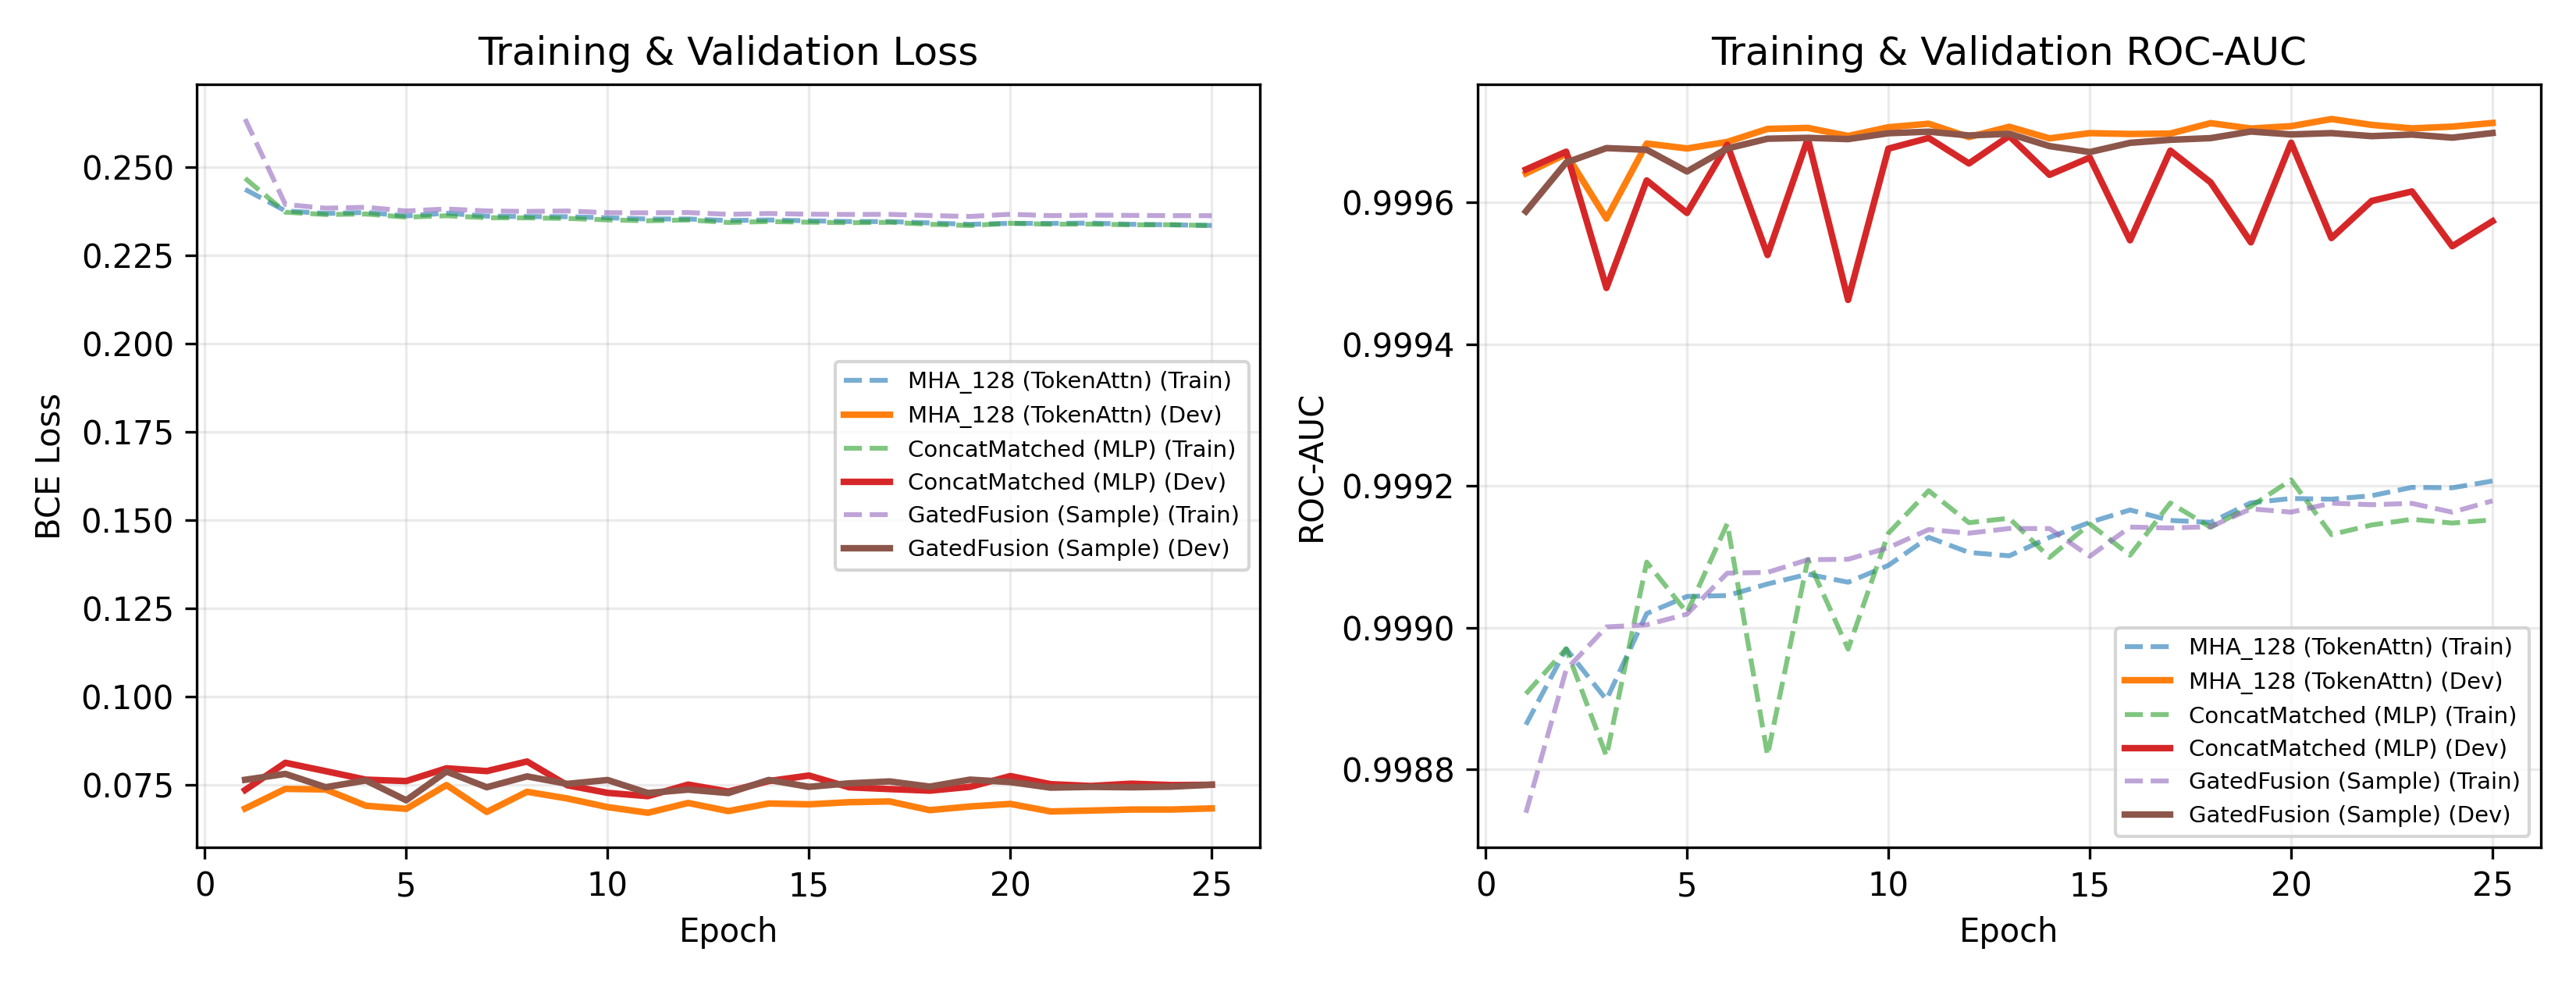
\includegraphics[width=0.96\linewidth]{figures/fig2_train_val_convergence.png}
\caption{Cross-fitted Phase 2 training (dashed) and held-out \texttt{fusion\_dev} (solid) BCE loss and ROC-AUC convergence curves over 25 epochs (seed 42). Training BCE loss sits above validation BCE loss because training uses label smoothing ($s=0.05$, floor $\approx 0.199$), modality dropout ($p=0.15$), and forensic augmentations while \texttt{fusion\_dev} is evaluated cleanly on hard labels. \texttt{MHA\_128} achieves the lowest and most stable validation loss and ROC-AUC.}
\label{fig:convergence}
\end{figure}

Table~\ref{tab:seen_test} reports exact, programmatically verified metrics on the untouched \texttt{seen\_test} split ($n=12,729$: 6,515 real, 6,214 fake), including raw seed-42 confusion counts, a single consistent Macro-F1 definition ($\text{Macro-F1} = \frac{1}{2}(\text{F1}_{\text{real}}+\text{F1}_{\text{fake}})$), and probability calibration metrics (Brier score and 15-bin ECE), while Appendix Table~\ref{tab:stats_appendix} provides the complete identity-cluster bootstrap 95\% confidence intervals, all four unrounded per-seed scores, Holm--Bonferroni $p$-values, and paired Cohen's $d$ effect sizes. Both standalone experts perform strongly (\texttt{Wang2020\_128}: 98.76\% accuracy, 1.12\% EER, 99.55\% authentic recall / 29 FPs, 97.92\% synthetic recall / 129 FNs; \texttt{Wolter2021\_128}: 97.53\% accuracy, 2.40\% EER, 98.62\% authentic recall / 90 FPs, 96.40\% synthetic recall / 224 FNs). Every two-stream fusion architecture decisively outperforms both standalone experts overall: \texttt{MHA\_128} elevates accuracy to $99.12\% \pm 0.01\%$ across 4 seeds (seed 42: $99.14\%$, $\text{TN}=6,480$, $\text{FP}=35$, $\text{FN}=75$, $\text{TP}=6,139$, exact $(6480+6139)/12729=99.1358\%$), improves ROC-AUC to $0.9997$, lowers EER from 1.12\%/2.40\% to $0.87\% \pm 0.03\%$, and lowers Brier score from $0.0126$/$0.0185$ to $0.0084$. Reporting both directions of the authentic-vs-synthetic trade-off transparently: relative to \texttt{Wolter2021\_128}, \texttt{MHA\_128} reduces false positives by 61.1\% ($90 \to 35$, lifting authentic recall $98.62\% \to 99.46\%$) and false negatives by 66.5\% ($224 \to 75$); relative to \texttt{Wang2020\_128}, \texttt{MHA\_128} slashes spatial false negatives by 41.9\% ($129 \to 75$, lifting synthetic recall $97.92\% \to 98.79\%$) at the modest cost of 6 additional false positives ($29 \to 35$, authentic recall $99.55\% \to 99.46\%$, $-0.09\%$).

Crucially, once capacity is matched ($\approx$199K parameters) and cross-fitting is enforced, paired four-seed $t$-tests with Holm--Bonferroni correction (Table~\ref{tab:stats_appendix}) confirm that \texttt{MHA\_128}, \texttt{ConcatMatchedMLP}, \texttt{NoAttnFFN}, and \texttt{LinearMix} are statistically indistinguishable on in-domain \texttt{seen\_test} accuracy and EER (all $p_{\text{Holm}} \ge 0.15$; accuracy spread $99.10\%$--$99.16\%$, all ROC-AUC $=0.9997$), while \texttt{MHA\_128} achieves a statistically significant Brier-score calibration improvement over both \texttt{GatedFusion} ($d=-8.69$, $p_{\text{Holm}}=0.0021$) and original \texttt{Fusion\_128} ($d=-4.13$, $p_{\text{Holm}}=0.0186$). This candid result directly answers the capacity-confound critique: on seen generators where both frozen embeddings are already highly separable, feed-forward refinement and capacity matching account for the bulk of in-domain fusion accuracy, whereas differences emerge in probability calibration, same-pipeline controls, and out-of-distribution generalization.

\begin{table}[tbp]
\centering
\caption{Programmatically verified evaluation on untouched held-out \texttt{seen\_test} ($n=12,729$: 6,515 Real, 6,214 Fake). Fusion rows report 4-seed Mean $\pm$ SD alongside exact seed-42 confusion counts (\texttt{TN/FP/FN/TP}). Seed-42 confusion counts reproduce seed-42 accuracies exactly (\texttt{MHA\_128}: 99.14\%, \texttt{ConcatMatchedMLP}: 99.10\%, \texttt{NoAttnFFN}: 99.13\%, \texttt{LinearMix}: 99.15\%, \texttt{GatedFusion}: 99.10\%, \texttt{Fusion\_128}: 99.10\%); see Table~\ref{tab:stats_appendix} for all 4 individual seeds and identity-cluster bootstrap 95\% CIs.}
\label{tab:seen_test}
\scriptsize
\begin{tabular}{@{}lrrrrrrrr@{}}
\toprule
\textbf{Model} & \textbf{Params} & \textbf{Acc (\%)} & \textbf{Macro-F1} & \textbf{ROC-AUC} & \textbf{EER (\%)} & \textbf{Brier} & \textbf{ECE} & \textbf{Seed-42 CM (TN/FP/FN/TP)} \\
\midrule
\texttt{Wang2020\_128} (RGB) & 23.77M & 98.76 & 0.9876 & 0.9995 & 1.12 & 0.0126 & 0.0574 & 6486 / 29 / 129 / 6085 \\
\texttt{Wolter2021\_128} (Freq) & 1.73M & 97.53 & 0.9753 & 0.9976 & 2.40 & 0.0185 & \textbf{0.0110} & 6425 / 90 / 224 / 5990 \\
\texttt{Xception} (ICCV 2019 \cite{ref12,ref28}) & 20.81M & 99.18 & --- & 0.9995 & 0.63 & --- & --- & External Baseline \\
\texttt{UniversalFakeDetect} (CVPR 2023 \cite{ref41}) & 304M* & 98.05 & --- & 0.9979 & 2.01 & --- & --- & Frozen CLIP Linear Probe \\
\midrule
\texttt{MHA\_128} (TokenAttn) & 199,425 & 99.12$\pm$0.01 & 0.9912 & \textbf{0.9997} & 0.87$\pm$0.03 & 0.0084 & 0.0473 & 6480 / 35 / \textbf{75} / \textbf{6139} \\
\texttt{ConcatMatchedMLP} & 198,017 & 99.13$\pm$0.02 & 0.9913 & \textbf{0.9997} & 0.86$\pm$0.02 & 0.0089 & 0.0505 & 6481 / 34 / 80 / 6134 \\
\texttt{NoAttnFFN} & 198,657 & 99.13$\pm$0.07 & 0.9913 & \textbf{0.9997} & 0.83$\pm$0.02 & 0.0083 & 0.0455 & 6482 / 33 / 78 / 6136 \\
\texttt{LinearMix} & 198,785 & \textbf{99.16$\pm$0.06} & \textbf{0.9916} & \textbf{0.9997} & \textbf{0.81$\pm$0.01} & \textbf{0.0082} & 0.0459 & 6490 / 25 / 83 / 6131 \\
\texttt{GatedFusion} & 41,987 & 99.10$\pm$0.00 & 0.9910 & \textbf{0.9997} & 0.92$\pm$0.01 & 0.0094 & 0.0534 & 6483 / 32 / 83 / 6131 \\
\texttt{Fusion\_128} (Orig) & 107,009 & 99.11$\pm$0.02 & 0.9911 & \textbf{0.9997} & 0.90$\pm$0.02 & 0.0092 & 0.0537 & 6484 / 31 / 84 / 6130 \\
\bottomrule
\end{tabular}
\end{table}

\subsection*{Per-Source Recall, Per-Generator Decomposition, and Strictly Native PNG-Only Control}
Table~\ref{tab:per_gen} decomposes untouched \texttt{seen\_test} performance individually across all three authentic sources and all thirteen seen generators, together with a strictly same-pipeline control restricting both classes exclusively to native PNG imagery (\texttt{FFHQ-256} + \texttt{FairFace} reals, $n=3,515$, vs.\ all PNG fakes, $n=6,214$). Note that the revised benchmark evaluates high-resolution still-image diffusion and face-swap generators rather than compressed FaceForensics++ video frames (hence FF++ manipulation-type video subsets are excluded by design, while the published FF++ \texttt{Xception} detector is benchmarked directly in Tables~\ref{tab:seen_test} and \ref{tab:unseen}). On the strictly PNG-only control, \textbf{\texttt{MHA\_128} ranks first across every metric}: $0.9996$ ROC-AUC, $98.90\%$ accuracy, $98.94\%$ balanced accuracy, $0.9881$ Macro-F1, $1.04\%$ EER, $0.0098$ Brier score, and $0.0458$ ECE---surpassing \texttt{Wang2020\_128} ($98.49\%$, $1.19\%$ EER), \texttt{Wolter2021\_128} ($96.93\%$, $2.87\%$ EER), \texttt{ConcatMatchedMLP} ($98.85\%$, $1.08\%$ EER), and \texttt{GatedFusion} ($98.85\%$, $1.11\%$ EER). Across individual generators, fusion yields the largest gains on the hardest pixel-diffusion models: on ADM, recall rises from $92.3\%$ (RGB) and $89.5\%$ (Wavelet) to \textbf{$96.8\%$ (\texttt{MHA\_128})}; on \texttt{cycle\_diff}, from $91.3\%$ / $84.3\%$ to \textbf{$92.5\%$}, and on \texttt{DreamBooth} from $97.5\%$ / $96.4\%$ to \textbf{$98.6\%$}.

\begin{table}[tbp]
\centering
\caption{Individual per-source authentic recall, per-generator synthetic recall / ROC-AUC across all 13 seen generators on untouched \texttt{seen\_test} (seed 42), and strictly native PNG-only same-pipeline control ($n=3,515$ PNG reals vs.\ $6,214$ PNG fakes). Per-generator decomposition was logged for the four primary models (\texttt{Wang2020\_128}, \texttt{Wolter2021\_128}, \texttt{ConcatMatched}, \texttt{MHA\_128}); \texttt{GatedFusion} is additionally reported on all three real sources and the PNG-only control.}
\label{tab:per_gen}
\scriptsize
\begin{tabular}{@{}lrrrrr@{}}
\toprule
\textbf{Subset / Generator ($n$)} & \textbf{\texttt{Wang2020\_128}} & \textbf{\texttt{Wolter2021\_128}} & \textbf{\texttt{ConcatMatched}} & \textbf{\texttt{GatedFusion}} & \textbf{\texttt{MHA\_128}} \\
\midrule
\multicolumn{6}{@{}l}{\textit{Authentic Recall (\%) Stratified by Source Dataset}} \\
CelebA (3,000, JPG) & 99.63\% & 99.50\% & \textbf{99.93\%} & 99.90\% & 99.90\% \\
FairFace Val (1,415, PNG) & \textbf{100.00\%} & 99.93\% & 99.93\% & 99.93\% & 99.93\% \\
FFHQ-256 (2,100, PNG) & \textbf{99.14\%} & 96.48\% & 98.52\% & 98.67\% & 98.52\% \\
\midrule
\multicolumn{6}{@{}l}{\textit{Individual Synthetic Recall (\%) / ROC-AUC per Seen Generator (vs.\ All 6,515 Held-Out Reals)}} \\
ADM (750) & 92.3\% / 0.9983 & 89.5\% / 0.9942 & 96.5\% / 0.9991 & --- & \textbf{96.8\% / 0.9991} \\
DDPM (750) & \textbf{99.9\% / 1.0000} & 98.9\% / 0.9993 & \textbf{99.9\% / 1.0000} & --- & \textbf{99.9\% / 1.0000} \\
DDIM (750) & \textbf{99.9\% / 1.0000} & 99.1\% / 0.9995 & \textbf{99.9\% / 1.0000} & --- & \textbf{99.9\% / 1.0000} \\
DiffSwap (750) & 97.3\% / 0.9992 & 96.7\% / 0.9981 & 98.4\% / 0.9996 & --- & \textbf{98.5\% / 0.9996} \\
CoDiff (393) & 100.0\% / 0.9999 & 99.7\% / 0.9998 & \textbf{100.0\% / 1.0000} & --- & \textbf{100.0\% / 1.0000} \\
cycle\_diff (415) & 91.3\% / 0.9982 & 84.3\% / 0.9893 & 92.3\% / 0.9986 & --- & \textbf{92.5\% / 0.9986} \\
DCFace (402) & \textbf{100.0\% / 1.0000} & \textbf{100.0\% / 1.0000} & \textbf{100.0\% / 1.0000} & --- & \textbf{100.0\% / 1.0000} \\
DreamBooth (363) & 97.5\% / 0.9990 & 96.4\% / 0.9935 & 98.3\% / 0.9996 & --- & \textbf{98.6\% / 0.9997} \\
FreeDoM\_I (333) & \textbf{100.0\% / 1.0000} & 99.4\% / 0.9997 & \textbf{100.0\% / 1.0000} & --- & \textbf{100.0\% / 1.0000} \\
FreeDoM\_T (296) & \textbf{100.0\% / 1.0000} & 99.7\% / 0.9998 & \textbf{100.0\% / 1.0000} & --- & \textbf{100.0\% / 1.0000} \\
HPS (408) & 99.3\% / 0.9998 & 96.8\% / 0.9978 & 99.5\% / 0.9998 & --- & \textbf{99.8\% / 0.9998} \\
LoRA (207) & \textbf{100.0\% / 1.0000} & 99.0\% / 0.9992 & \textbf{100.0\% / 1.0000} & --- & \textbf{100.0\% / 1.0000} \\
SDXL (397) & 99.7\% / 1.0000 & 98.0\% / 0.9993 & \textbf{100.0\% / 1.0000} & --- & 99.7\% / 1.0000 \\
\midrule
\multicolumn{6}{@{}l}{\textit{Same-Pipeline Control: Strictly Native PNG Reals (3,515) vs.\ Native PNG Fakes (6,214)}} \\
Accuracy / Balanced Acc & 98.49\% / 98.71\% & 96.93\% / 97.13\% & 98.85\% / 98.90\% & 98.85\% / 98.92\% & \textbf{98.90\% / 98.94\%} \\
ROC-AUC / EER / Brier & 0.9994 / 1.19\% / 0.0150 & 0.9965 / 2.87\% / 0.0230 & 0.9995 / 1.08\% / 0.0107 & 0.9995 / 1.11\% / 0.0112 & \textbf{0.9996 / 1.04\% / 0.0098} \\
\bottomrule
\end{tabular}
\end{table}

\subsection*{Unseen Cross-Domain Generalization, Joint-Training Control, and Capacity Sweep}
Table~\ref{tab:unseen} and Figure~\ref{fig:ablation_bars} evaluate zero-tuning cross-domain transfer across four completely unseen photorealistic domains under matched JPEG $Q=85$ recompression (1,000 unseen LFW camera reals vs.\ 1,000 unseen fakes per generator). Three important findings emerge:

\begin{enumerate}
    \item \textbf{Empirical Proof of Staged Decoupling vs.\ Joint End-to-End Training:} Under a compute-constrained verification budget (80,000 balanced LOGO training images, 2 epochs---also used for our supplementary \texttt{Xception} and \texttt{ConvNeXt\_128} controls), training the exact same ResNet-50 + Wavelet CNN + \texttt{MHA\_128} pipeline \emph{jointly unfrozen} end-to-end severely collapsed on unseen real camera imagery (\texttt{LFW} real recall $=4.5\%$, unseen accuracy $=52.10\%$ on LDM/DiffFace, $52.15\%$ on SDXL\_Refine, and $12.20\%$ / $0.0515$ AUC on StyleGAN). By contrast, staged decoupled training preserved $90.3\%$--$98.5\%$ unseen real recall and $83.35\%$--$85.71\%$ four-domain unseen mean accuracy ($0.865$--$0.957$ mean AUC), empirically motivating staged decoupling (while acknowledging that full 439K-image joint training with explicit gradient balancing remains an open future test).
    \item \textbf{Sample-Dependent Weighting Works---and Lightweight Gating Generalizes Best Under Shift:} Both sample-dependent heads dynamically modulate modality weights per domain: \texttt{GatedFusion} shifts its gate from \textbf{23.1\% RGB / 76.9\% Wavelet} on authentic LFW photos to \textbf{79.0\%--83.7\% RGB / 16.3\%--21.0\% Wavelet} on unseen diffusion fakes (LDM, SDXL\_Refine, DiffFace) and \textbf{63.5\% RGB / 36.5\% Wavelet} on StyleGAN. Similarly, \texttt{MHA\_128}'s $[\text{CLS}]$ token shifts attention from \textbf{33.0\% RGB / 38.1\% Wavelet} on LFW reals to \textbf{38.5\%--39.5\% RGB / 27.1\%--31.0\% Wavelet} on LDM/DiffFace and \textbf{46.2\% RGB / 19.0\% Wavelet} on StyleGAN. Across all four seeds, \textbf{\texttt{GatedFusion} (41,987 parameters) achieves the strongest four-domain unseen mean accuracy} ($85.71\% \pm 0.06\%$ vs.\ $84.84\%$ for standalone \texttt{Wolter2021\_128} and $83.35\%$ for \texttt{Wang2020\_128}, $0.9164 \pm 0.0150$ mean AUC, $11.46\%$ EER, and \textbf{95.40\% accuracy / 0.9907 AUC on unseen DiffFace swaps}, beating both standalone experts by $+2.55\%$ to $+5.40\%$). Transparently, standalone \texttt{Wolter2021\_128} retains the highest 4-domain mean ROC-AUC ($0.9568$ vs.\ $0.9164$) specifically because its high-frequency features rank zero-shot StyleGAN fakes strongly ($0.8411$ AUC vs.\ $0.5171$ for RGB and $0.5785$--$0.7229$ for fusion), whereas \texttt{GatedFusion} leads 4-domain operating-point accuracy at $\tau=0$. Meanwhile, \texttt{MHA\_128} outperforms both \texttt{NoAttnFFN} ($84.71\%$ vs.\ $84.06\%$) and \texttt{LinearMix} ($83.65\%$) and achieves the \textbf{lowest probability calibration error} on pooled unseen diffusion+swap ($\text{ECE}=0.039$ vs.\ $0.049$ for \texttt{ConcatMatchedMLP}, $0.062$ for RGB, and $0.076$ for Wavelet; Figure~\ref{fig:roc_pr_rel}), while trailing \texttt{GatedFusion} and \texttt{ConcatMatchedMLP} slightly on unseen accuracy due to higher seed variance ($\pm 0.92\%$ vs.\ $\pm 0.06\%$; all Holm-corrected paired $p>0.34$, Table~\ref{tab:stats_appendix}).
    \item \textbf{External Published Baselines (\texttt{Xception} \& \texttt{UniversalFakeDetect}) and Honest Cross-Paradigm Boundary:} On identical splits (Tables~\ref{tab:seen_test} and \ref{tab:unseen}), fine-tuned \texttt{Xception} (FaceForensics++ \cite{ref12,ref28}, 80K balanced LOGO training, 2 epochs) achieves strong in-domain accuracy ($99.18\%$, $0.63\%$ EER) yet collapses severely on unseen camera photographs (LFW real recall $=7.0\%$, unseen 4-domain mean accuracy $=43.04\%$). Conversely, \texttt{UniversalFakeDetect} (Ojha et al.\ \cite{ref41}, frozen 304M CLIP ViT-L/14 linear probe) achieves $98.05\%$ on \texttt{seen\_test} ($2.01\%$ EER) and $68.90\%$ on unseen StyleGAN ($0.7636$ AUC), yet our 12$\times$ smaller 25.5M \texttt{GatedFusion} outperforms \texttt{UniversalFakeDetect} on \texttt{seen\_test} ($99.10\%$ vs.\ $98.05\%$) and on \textbf{all three unseen diffusion/swap benchmarks} (\texttt{LDM} $96.45\%$ vs.\ $94.95\%$, \texttt{SDXL\_Refine} $97.35\%$ vs.\ $95.30\%$, \texttt{DiffFace} $95.40\%$ vs.\ $94.90\%$, LFW real recall $94.8\%$ vs.\ $91.2\%$). Recent 2025--2026 architectures discussed in Related Work (FAViT \cite{ref43}, LGF-Net \cite{ref44}, FreqDebias \cite{ref45}) are cited for literature positioning rather than experimentally re-implemented, and we make no direct empirical superiority claim over them. With zero GANs in training, \texttt{Wang2020\_128} collapses to near-chance on StyleGAN ($0.5171$ AUC, $50.70\%$ accuracy), whereas \texttt{Wolter2021\_128} retains $0.8411$ AUC (surpassing even CLIP's $0.7636$ AUC). A 16-configuration width/dropout sweep of the concatenation MLP ($\text{width}\in\{128,256,384,512\}$, $\text{dropout}\in\{0.1,0.2,0.3,0.5\}$; 41.7K--263.7K parameters; Table~\ref{tab:stats_appendix}) confirmed tight stability across all settings (\texttt{seen\_test} AUC $0.99966$--$0.99969$; unseen 4-domain mean accuracy $85.08\%$--$85.51\%$, mean AUC $0.8810$--$0.9148$), ruling out baseline under-tuning.
\end{enumerate}

\begin{table}[tbp]
\centering
\caption{Zero-tuning unseen cross-domain generalization under standardized JPEG $Q=85$ recompression (1,000 unseen LFW camera reals vs.\ 1,000 unseen fakes per generator). Top block: individual domain seed-42 AUC / Acc (\%). Bottom columns: 4-seed Mean $\pm$ SD across all 4 unseen domains.}
\label{tab:unseen}
\scriptsize
\begin{tabular}{@{}lcccccc@{}}
\toprule
\textbf{Model} & \textbf{LDM} & \textbf{SDXL\_Refine} & \textbf{DiffFace (Swap)} & \textbf{StyleGAN (0 GANs)} & \textbf{4-Dom Mean AUC} & \textbf{4-Dom Mean Acc (\%)} \\
\midrule
\texttt{Wang2020\_128} (RGB) & 0.9779 / 94.20\% & 0.9910 / 95.65\% & 0.9731 / 92.85\% & 0.5171 / 50.70\% & 0.8648 & 83.35 \\
\texttt{Wolter2021\_128} (Freq) & \textbf{0.9967 / 96.50\%} & \textbf{0.9994 / 98.75\%} & 0.9901 / 90.00\% & \textbf{0.8411} / 54.10\% & \textbf{0.9568} & 84.84 \\
\texttt{Xception} (ICCV 2019 \cite{ref12,ref28}) & 0.9605 / 53.35\% & 0.9859 / 53.45\% & 0.9764 / 53.50\% & 0.0819 / 11.85\% & 0.7512 & 43.04 \\
\texttt{UniversalFakeDetect} (CVPR 2023 \cite{ref41}) & 0.9947 / 94.95\% & 0.9971 / 95.30\% & 0.9944 / 94.90\% & 0.7636 / \textbf{68.90\%} & 0.9375 & \textbf{88.51} \\
Joint E2E Unfrozen (Control) & 0.8861 / 52.10\% & 0.9172 / 52.15\% & 0.8586 / 52.10\% & 0.0515 / 12.20\% & 0.6784 & 42.14 \\
\midrule
\texttt{MHA\_128} (TokenAttn) & 0.9888 / 94.30\% & 0.9984 / 95.10\% & 0.9781 / 92.70\% & 0.5785 / 51.60\% & 0.9049$\pm$0.0211 & 84.71$\pm$0.92 \\
\texttt{ConcatMatchedMLP} & 0.9933 / 96.25\% & 0.9978 / 97.10\% & 0.9857 / 94.45\% & 0.6484 / 53.45\% & 0.9145$\pm$0.0080 & 85.36$\pm$0.39 \\
\texttt{NoAttnFFN} & 0.9908 / 95.70\% & 0.9986 / 96.65\% & 0.9816 / 94.05\% & 0.7229 / 52.95\% & 0.9085$\pm$0.0175 & 84.06$\pm$0.60 \\
\texttt{LinearMix} & 0.9862 / 94.20\% & 0.9957 / 95.10\% & 0.9717 / 92.25\% & 0.6227 / 51.20\% & 0.9044$\pm$0.0255 & 83.65$\pm$0.71 \\
\textbf{\texttt{GatedFusion} (Sample)} & 0.9950 / 96.45\% & 0.9992 / 97.35\% & \textbf{0.9907 / 95.40\%} & 0.6331 / 53.55\% & \textbf{0.9164$\pm$0.0150} & \textbf{85.71$\pm$0.06} \\
\texttt{Fusion\_128} (Orig) & 0.9939 / 96.05\% & 0.9987 / 97.00\% & 0.9874 / 94.30\% & 0.6228 / 53.10\% & 0.8973$\pm$0.0029 & 85.55$\pm$0.31 \\
\bottomrule
\end{tabular}
\end{table}

\subsection*{Backbone-Agnostic Modularity Verification (\texttt{ConvNeXt\_128} with Matched Fusion Controls)}
To verify that the decoupled fusion framework generalizes across modern spatial backbones---and to compare \texttt{MHA\_128} against matched \texttt{ConcatMatchedMLP} and \texttt{GatedFusion} controls on a second backbone---we trained \texttt{ConvNeXt\_128} (ConvNeXt-Base with a 128-D bottleneck, 80K balanced LOGO samples, 2 epochs) and cross-fitted all three fusion heads over the exact same frozen \texttt{Wolter2021\_128} embeddings across four seeds (Table~\ref{tab:convnext}). Standalone \texttt{ConvNeXt\_128} achieved $99.52\%$ on \texttt{seen\_test} ($0.49\%$ EER) yet overfit seen capture statistics, dropping to $49.62\%$ four-domain unseen mean accuracy ($0.7167$ AUC). Fusing with frozen \texttt{Wolter2021\_128} improved \emph{both} in-domain and unseen performance across all three heads: \texttt{seen\_test} accuracy rose to $99.57\%$--$99.61\%$ ($0.9999$ AUC, EER reduced from $0.49\%$ to $0.33\%$--$0.39\%$), and four-domain unseen mean accuracy jumped by $+6.92\%$ (\texttt{ConcatMatched}: $56.54\%$), $+9.30\%$ (\texttt{GatedFusion}: $58.92\%$), and \textbf{$+9.86\%$ (\texttt{MHA\_128}: $59.48\%$, surpassing \texttt{ConcatMatched} by $+2.94\%$ under domain shift)}.

\begin{table}[tbp]
\centering
\caption{Backbone-agnostic modularity verification using \texttt{ConvNeXt\_128} paired with frozen \texttt{Wolter2021\_128} across 4 seeds, reporting both matched concatenation and sample-dependent fusion controls on identical \texttt{seen\_test} and unseen JPEG $Q=85$ benchmarks.}
\label{tab:convnext}
\scriptsize
\begin{tabular}{@{}lcccccc@{}}
\toprule
\textbf{Model (\texttt{ConvNeXt\_128} Backbone)} & \textbf{SeenTest Acc} & \textbf{SeenTest AUC} & \textbf{SeenTest EER} & \textbf{UnseenQ85 4-Dom Acc} & \textbf{UnseenQ85 4-Dom AUC} & \textbf{Seed-42 SDXL\_Ref AUC/Acc} \\
\midrule
\texttt{ConvNeXt\_128} (Standalone) & 99.52\% & 0.9998 & 0.49\% & 49.62\% & 0.7167 & --- \\
\texttt{ConvNeXt} + \texttt{ConcatMatchedMLP} & \textbf{99.61\%} & \textbf{0.9999} & \textbf{0.33\%} & 56.54\% & 0.7445 & 0.9809 / 68.15\% \\
\texttt{ConvNeXt} + \texttt{GatedFusion} & 99.59\% & \textbf{0.9999} & 0.39\% & 58.92\% & \textbf{0.7452} & 0.9842 / \textbf{71.50\%} \\
\textbf{\texttt{ConvNeXt} + \texttt{MHA\_128}} & 99.57\% & \textbf{0.9999} & 0.38\% & \textbf{59.48\%} & 0.7386 & \textbf{0.9927} / 69.50\% \\
\bottomrule
\end{tabular}
\end{table}

\begin{figure}[tbp]
\centering
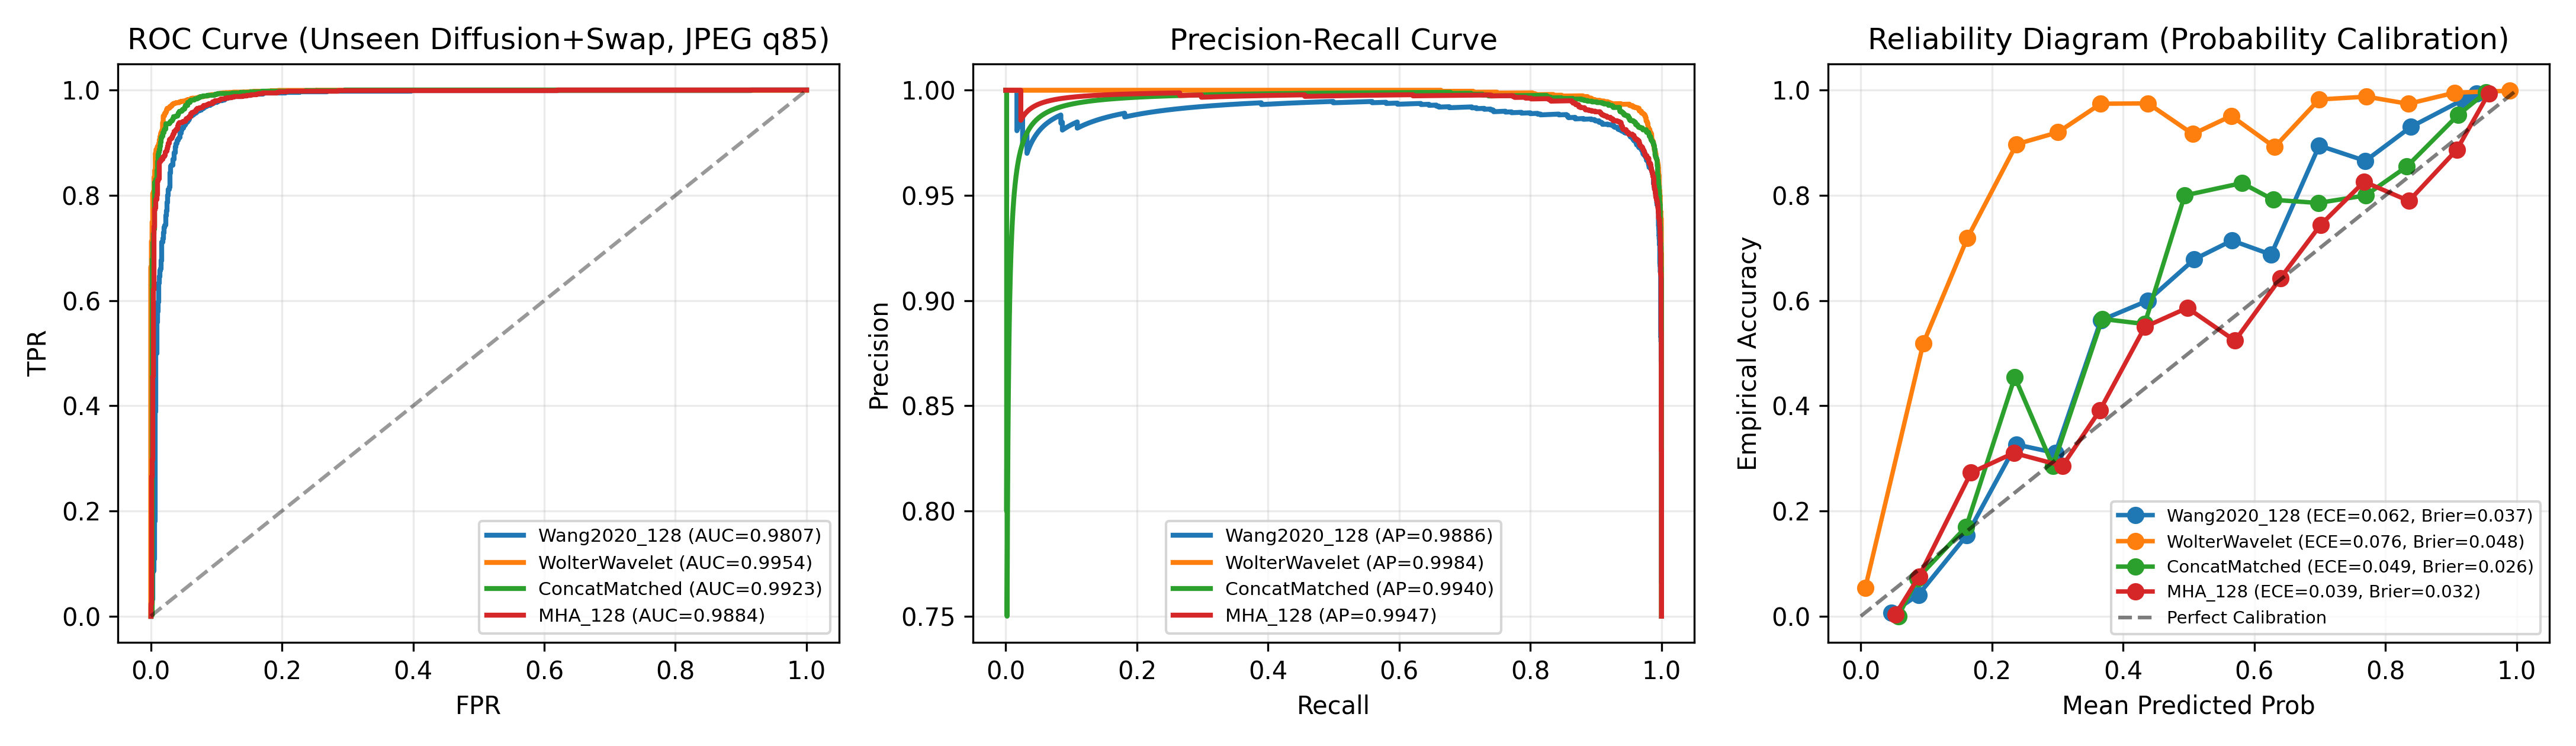
\includegraphics[width=\linewidth]{figures/fig3_roc_pr_reliability.png}
\caption{Pooled unseen diffusion and face-swap evaluation (1,000 LFW reals vs.\ 3,000 LDM + SDXL\_Refine + DiffFace fakes, JPEG $Q=85$): ROC curve, Precision--Recall curve, and 15-bin Reliability Diagram. \texttt{MHA\_128} achieves the closest alignment to the perfect-calibration diagonal ($\text{ECE}=0.039$).}
\label{fig:roc_pr_rel}
\end{figure}

\begin{figure}[tbp]
\centering
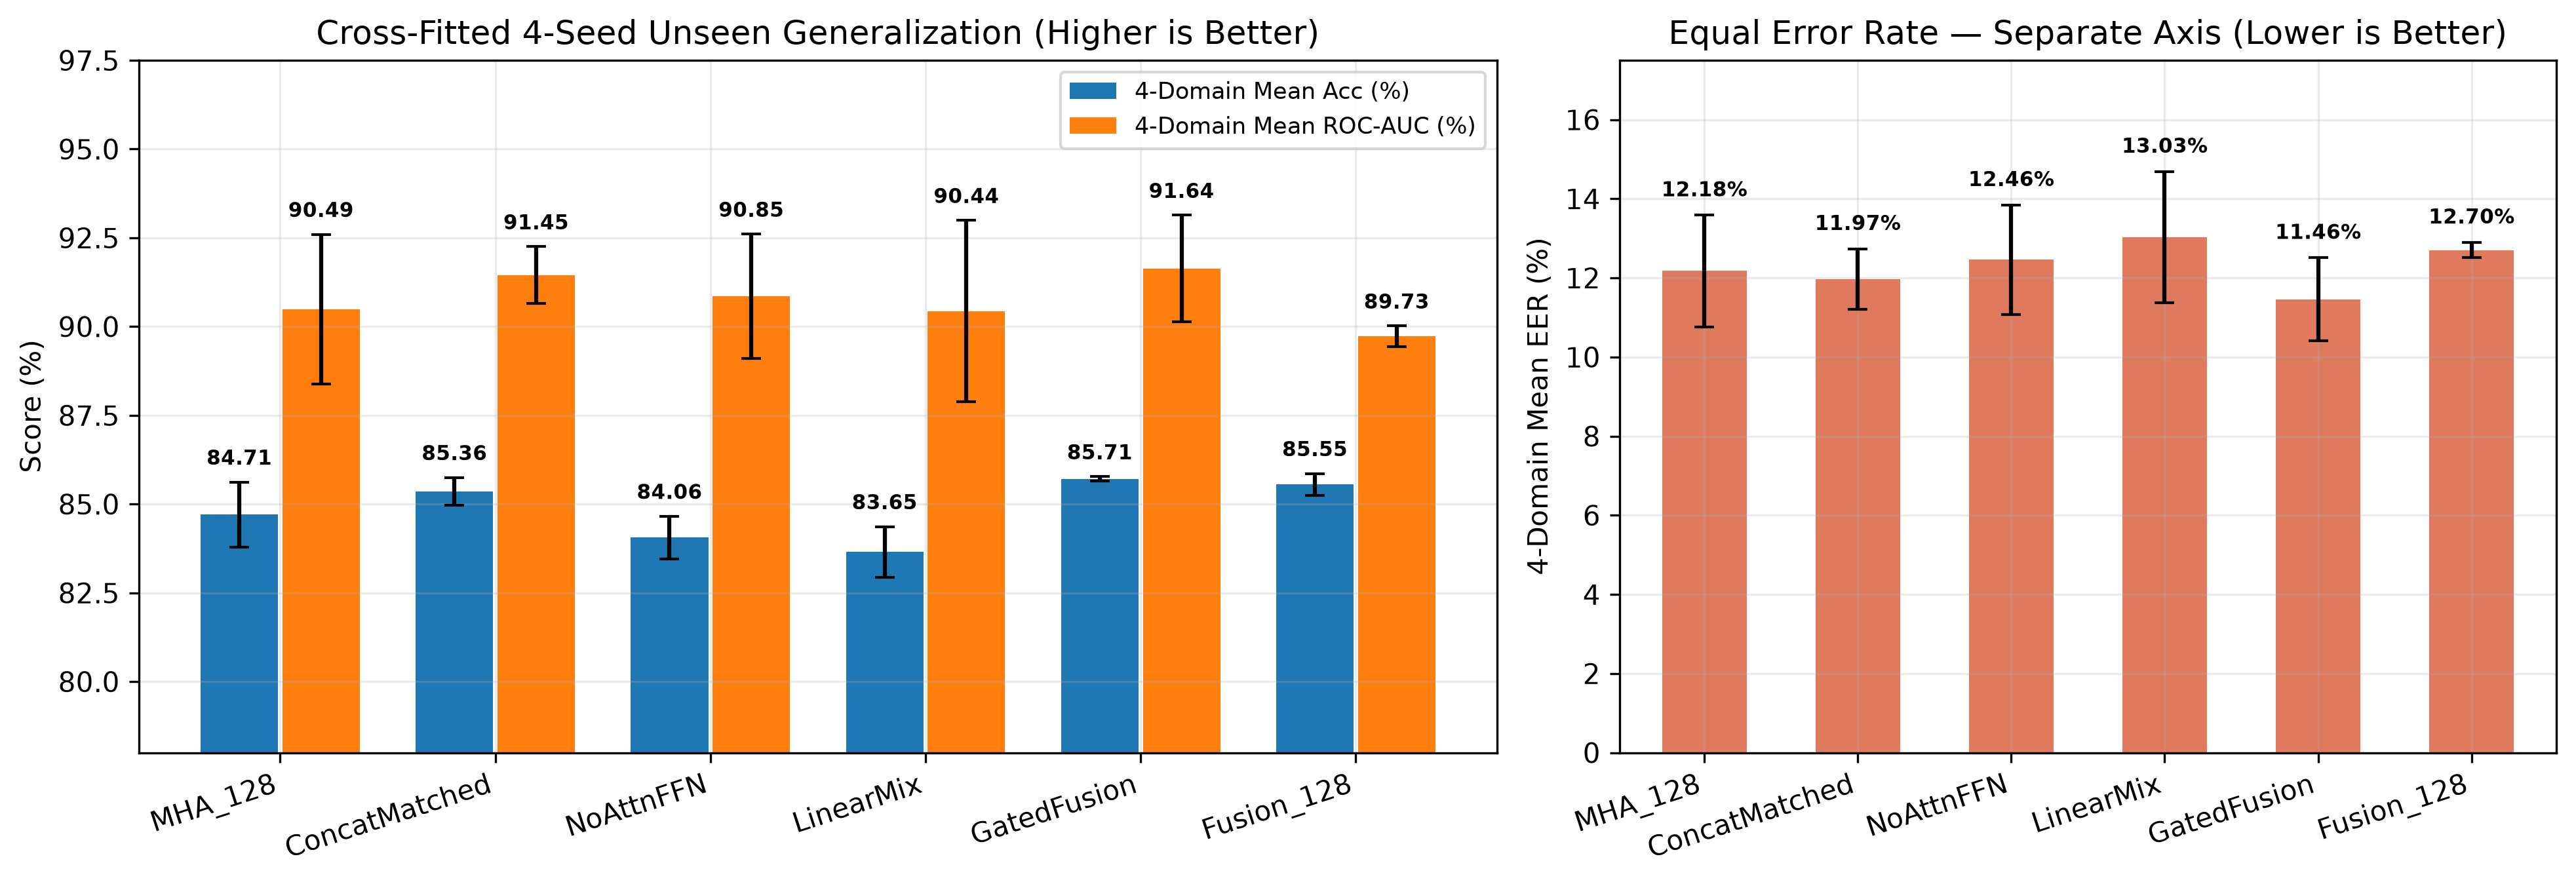
\includegraphics[width=\linewidth]{figures/fig4_ablation_4seed_bars.png}
\caption{Cross-fitted 4-seed unseen generalization across all six fusion architectures with explicit numeric labels, $\pm$SD error bars, and a dedicated Equal Error Rate (EER) axis (lower is better).}
\label{fig:ablation_bars}
\end{figure}

\subsection*{Real-World Perturbation Resilience, End-to-End FGSM Sweep, Fairness, and Latency}
\paragraph{Perturbation Robustness and Honest White-Box FGSM Vulnerability.}
Table~\ref{tab:robustness} and Figure~\ref{fig:robustness} evaluate all models on 500 unseen LFW reals vs.\ 500 unseen LDM fakes under nine real-world degradations and a matched white-box $L_\infty$ FGSM sweep ($\varepsilon \in \{0, 1/255, 2/255, 4/255, 8/255\}$; untargeted BCE loss maximization, raw $[0,1]$ pixel coordinates with $[0,1]$ clipping, zero random starts, gradients propagated end-to-end through ImageNet normalization and differentiable GPU Haar DWT). Under severe social-media compression and smoothing, two-stream fusion achieves strong synergy: \texttt{GatedFusion} reaches \textbf{97.7\% at JPEG $Q=30$}, \textbf{97.9\% at Blur $\sigma=2.0$}, and \textbf{96.1\% at $0.5\times$ downscaling}---beating both standalone experts on every severity. Conversely, two honest failure boundaries emerge: (i) additive white Gaussian noise ($\sigma=10$), deliberately absent from training augmentations, reduces all models to $40.3\%$--$52.1\%$ accuracy; and (ii) under faithful end-to-end raw-pixel white-box FGSM, \textbf{all five un-hardened models collapse even at $\varepsilon = 1/255$} ($\text{AUC} \le 0.090$, accuracy $\le 13.4\%$, real recall $\le 7.2\%$). Unlike single-branch or normalized-space attacks that can overstate robustness, end-to-end gradient propagation confirms that fusion alone does not confer white-box adversarial immunity without dedicated adversarial training.

\begin{table}[tbp]
\centering
\caption{Real-world degradation robustness and matched end-to-end raw-pixel white-box FGSM sweep (500 unseen LFW reals vs.\ 500 unseen LDM fakes; AUC / Acc\%). FGSM rows additionally list exact per-class Real/Fake recall \texttt{(R/F\%)} for all five models.}
\label{tab:robustness}
\scriptsize
\begin{tabular}{@{}lccccc@{}}
\toprule
\textbf{Condition} & \textbf{\texttt{Wang2020\_128}} & \textbf{\texttt{Wolter2021\_128}} & \textbf{\texttt{ConcatMatched}} & \textbf{\texttt{GatedFusion}} & \textbf{\texttt{MHA\_128}} \\
\midrule
Clean RAW & 0.9649 / 91.5\% & \textbf{0.9970 / 97.0\%} & 0.9831 / 95.7\% & 0.9907 / 95.9\% & 0.9826 / 93.1\% \\
JPEG $Q=90$ & 0.9851 / 95.1\% & 0.9974 / 96.9\% & 0.9934 / 97.5\% & \textbf{0.9957 / 97.6\%} & 0.9911 / 96.0\% \\
JPEG $Q=70$ & 0.9846 / 94.6\% & 0.9984 / 97.1\% & 0.9940 / 97.2\% & \textbf{0.9964 / 97.8\%} & 0.9913 / 95.5\% \\
JPEG $Q=50$ & 0.9852 / 94.9\% & 0.9985 / 96.4\% & 0.9941 / 97.4\% & \textbf{0.9961 / 97.7\%} & 0.9920 / 95.9\% \\
JPEG $Q=30$ (severe) & 0.9817 / 93.5\% & 0.9992 / 96.2\% & 0.9944 / 96.8\% & \textbf{0.9967 / 97.7\%} & 0.9915 / 94.9\% \\
Gaussian Blur $\sigma=1.0$ & 0.9656 / 91.1\% & \textbf{0.9951} / 94.8\% & 0.9857 / 94.8\% & 0.9890 / \textbf{95.0\%} & 0.9799 / 93.4\% \\
Gaussian Blur $\sigma=2.0$ & 0.9902 / 96.3\% & 0.9959 / 96.1\% & 0.9931 / \textbf{98.1\%} & \textbf{0.9955} / 97.9\% & 0.9904 / 96.6\% \\
Downscale $0.5\times$ & 0.9796 / 92.9\% & \textbf{0.9935} / 93.7\% & 0.9877 / 95.2\% & 0.9915 / \textbf{96.1\%} & 0.9832 / 93.8\% \\
Gauss Noise $\sigma=10$ (unseen) & 0.2315 / 40.3\% & \textbf{0.5079 / 52.1\%} & 0.3292 / 44.1\% & 0.3081 / 42.9\% & 0.2831 / 42.1\% \\
\midrule
FGSM $\varepsilon = 1/255$ & 0.0069 / 6.1\% (0.2/12.0) & 0.0000 / 0.2\% (0.2/0.2) & 0.0901 / 13.4\% (3.8/23.0) & 0.0098 / 6.3\% (7.2/5.4) & 0.0059 / 3.9\% (0.6/7.2) \\
FGSM $\varepsilon = 2/255$ & 0.0078 / 5.5\% (0.8/10.2) & 0.0000 / 0.3\% (0.0/0.6) & 0.0371 / 8.9\% (0.8/17.0) & 0.0042 / 3.9\% (2.6/5.2) & 0.0021 / 1.8\% (0.2/3.4) \\
FGSM $\varepsilon = 4/255$ & 0.0101 / 4.9\% (0.8/9.0) & 0.0000 / 5.1\% (0.0/10.2) & 0.0124 / 8.2\% (0.8/15.6) & 0.0014 / 2.8\% (0.4/5.2) & 0.0008 / 1.3\% (0.0/2.6) \\
FGSM $\varepsilon = 8/255$ & 0.0133 / 5.5\% (0.2/10.8) & 0.0000 / 27.6\% (0.0/55.2) & 0.0066 / 15.9\% (0.0/31.8) & 0.0005 / 3.3\% (0.0/6.6) & 0.0005 / 2.8\% (0.0/5.6) \\
\bottomrule
\end{tabular}
\end{table}

\begin{figure}[tbp]
\centering
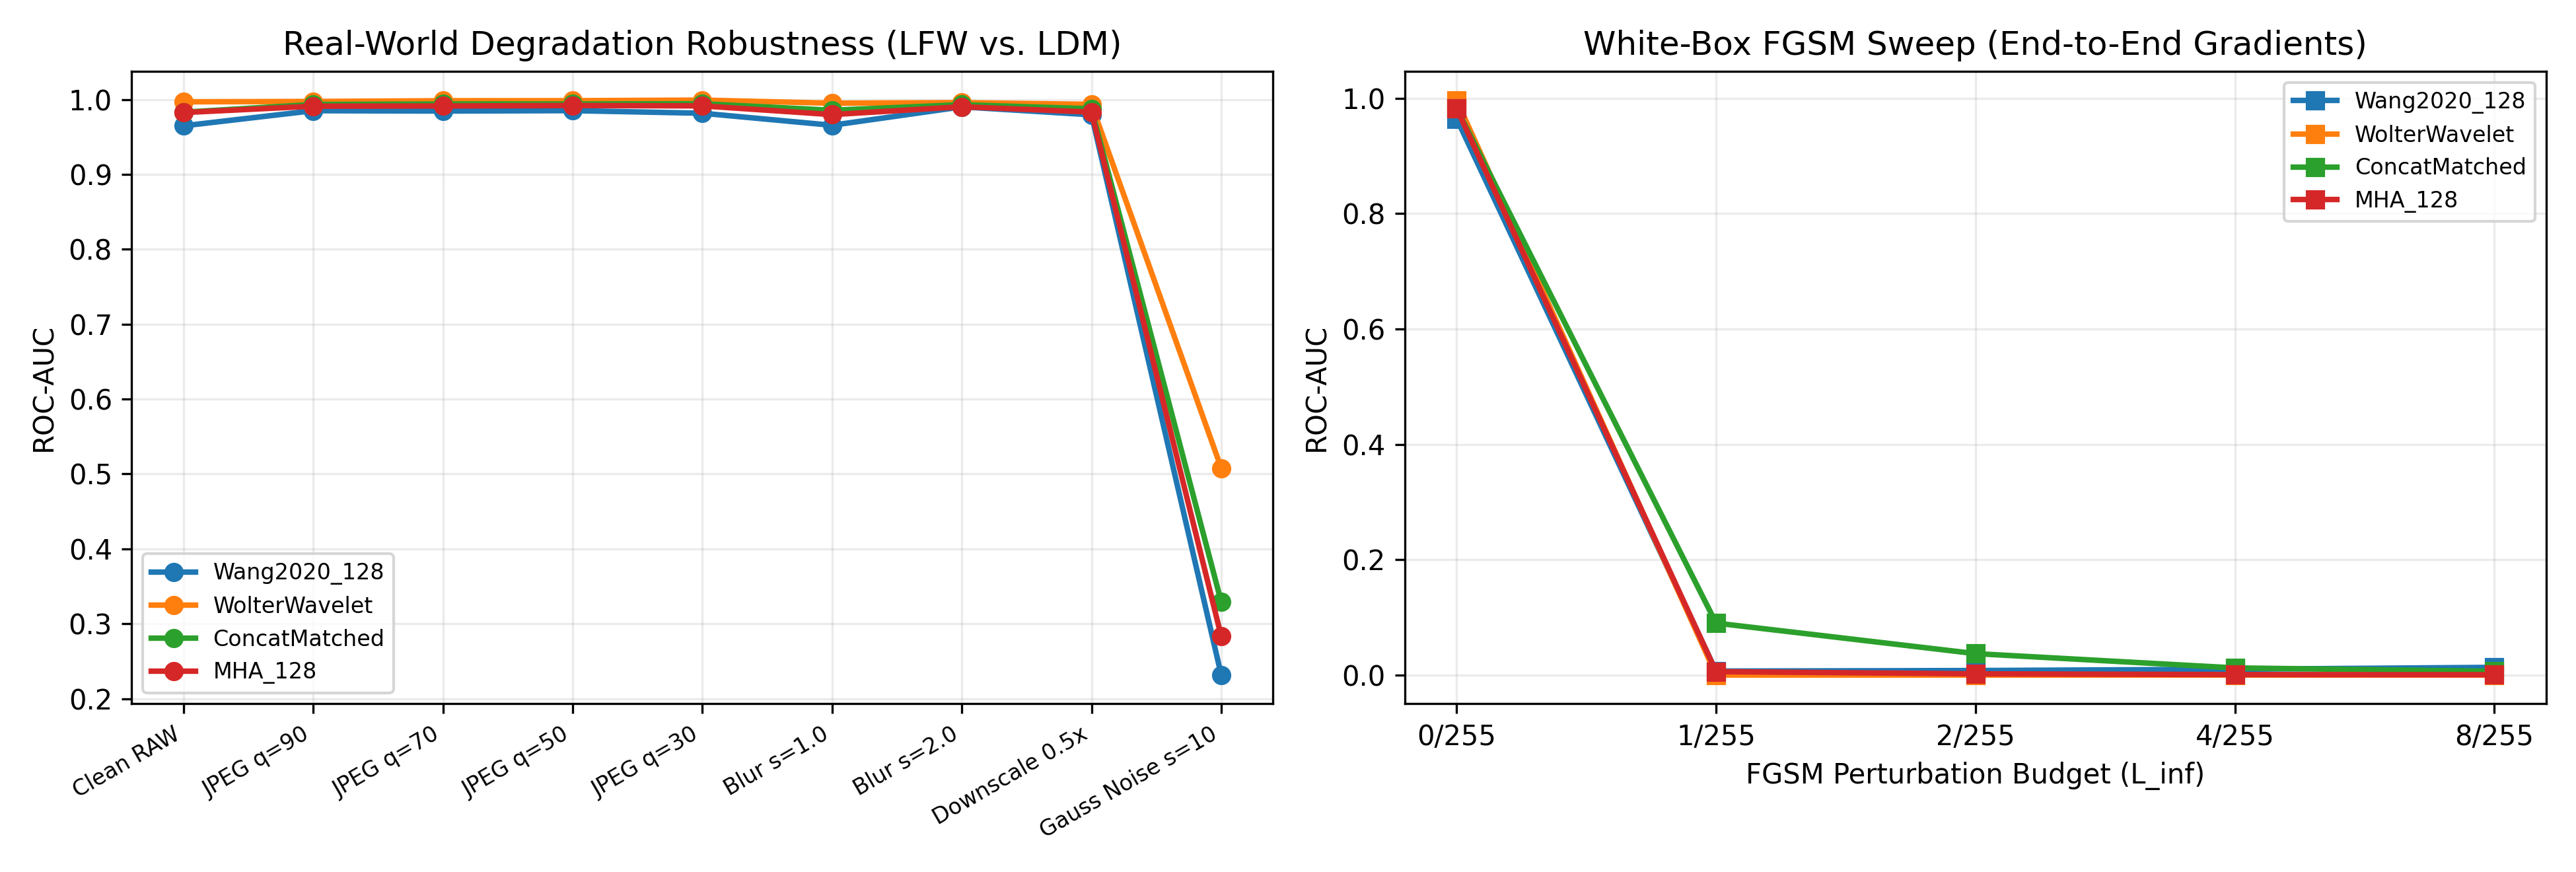
\includegraphics[width=\linewidth]{figures/fig5_robustness_perturb_fgsm.png}
\caption{Left: Real-world degradation resilience across compression, blur, downscaling, and unseen additive Gaussian noise (LFW vs.\ LDM). Right: Matched white-box end-to-end raw-pixel FGSM sweep across $\varepsilon \in [0, 8/255]$ confirming uniform vulnerability without adversarial training.}
\label{fig:robustness}
\end{figure}

\paragraph{Ground-Truth Demographic Fairness Audit (FairFace Validation, $n=2,000$).}
Using official ground-truth annotations on 2,000 identity-disjoint held-out FairFace validation faces spanning seven racial groups (Black 322, East Asian 304, Indian 242, Latino\_Hispanic 281, Middle Eastern 214, Southeast Asian 246, White 391), two genders (Female 935, Male 1,065), and nine age bands ($0$--$2$ through $>70$), \texttt{Wolter2021\_128}, \texttt{Fusion\_128}, and \texttt{MHA\_128} each achieved \textbf{$0.00\%$ false-positive rate ($\Delta\text{FPR}=0.00\%$)} across every single demographic subgroup, while \texttt{Wang2020\_128} achieved $\Delta\text{FPR} \le 0.33\%$ (East Asian $0.33\%$, Male $0.09\%$, Age 20--29 $0.17\%$, all others $0.00\%$). We note transparently that while FairFace validation is identity-disjoint from training, it shares FairFace's capture pipeline; on completely unseen LFW camera photographs, \texttt{GatedFusion} and \texttt{MHA\_128} exhibit $5.2\%$ and $7.5\%$ overall FPR, respectively.

\paragraph{Exact Latency Profiling Including Wavelet Preprocessing.}
Measured at batch size 1 in FP32 on an NVIDIA L4 GPU (30 warm-up, 200 timed iterations), \texttt{Wang2020\_128} requires $7.13\,$ms, the GPU 3-level Haar WPD transform requires $15.56\,$ms, \texttt{Wolter2021\_128} CNN inference requires $0.97\,$ms excluding DWT ($16.70\,$ms including DWT), and the \texttt{MHA\_128} fusion head requires only $0.76\,$ms---yielding a complete end-to-end dual-stream latency of \textbf{$24.92\,$ms per image ($\approx 40$ FPS) including GPU wavelet preprocessing}.

\subsection*{Quantitative Latent Separability and Grad-CAM Masking Controls}
Figure~\ref{fig:tsne} presents a single-row t-SNE projection ($n=400$ per domain, perplexity 30, PCA init, unseen JPEG $Q=85$) annotated with quantitative separability metrics on unit-normalized 128-D embeddings. Authentic LFW faces (green) separate cleanly from unseen diffusion generators across all three streams; \texttt{MHA\_128} achieves the largest inter-class Euclidean centroid distance ($1.284$ vs.\ $0.909$ RGB and $0.990$ Wavelet) with comparable Silhouette score ($0.367$ vs.\ $0.369$ RGB and $0.352$ Wavelet), while StyleGAN (blue) remains partially adjacent to real camera imagery for ResNet-50, visually explaining its cross-paradigm recall gap.

\begin{figure}[tbp]
\centering
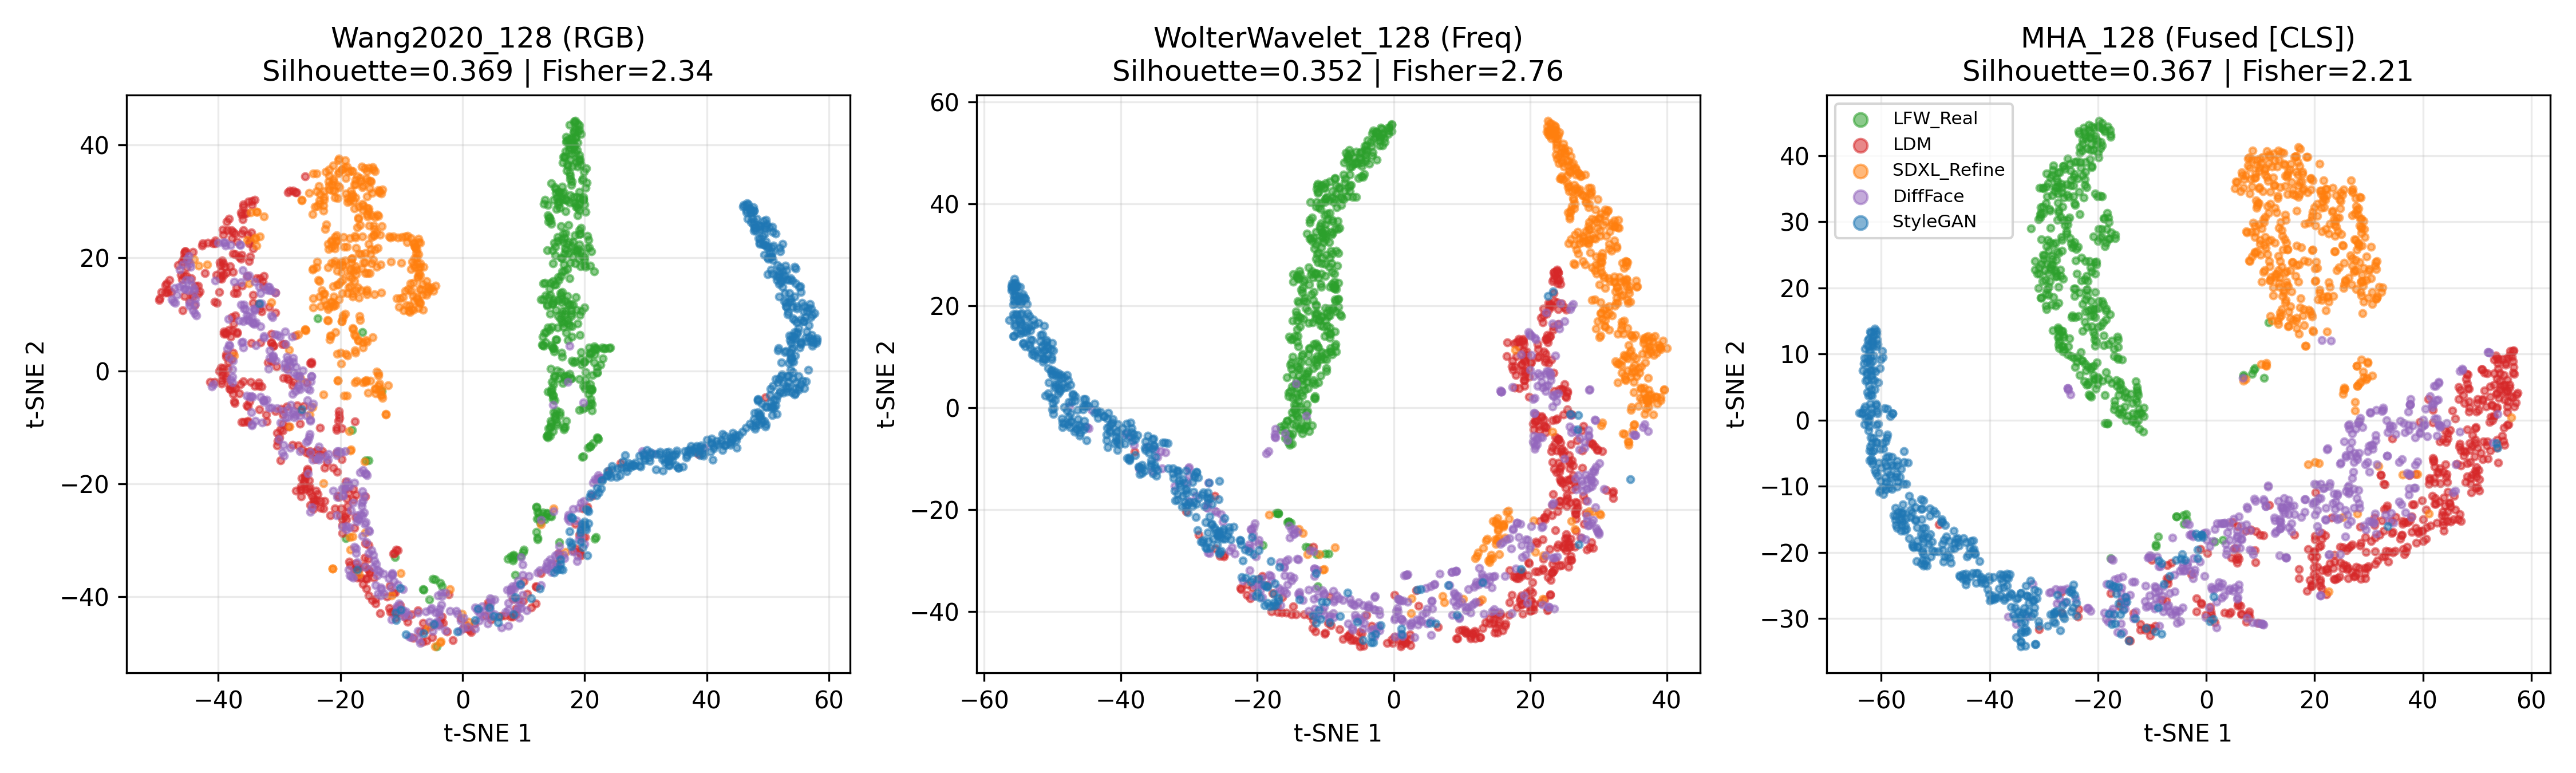
\includegraphics[width=\linewidth]{figures/fig6_tsne_silhouette.png}
\caption{Single-row t-SNE projections ($n=2,000$: 400 per unseen domain, JPEG $Q=85$, perplexity 30) with quantitative Silhouette scores and Fisher separation ratios computed on 128-D embeddings.}
\label{fig:tsne}
\end{figure}

Figure~\ref{fig:gradcam} presents ResNet-50 Layer 4 Grad-CAM maps with an explicit $[0,1]$ attribution scale across three unseen synthetic male face domains (LDM diffusion, DiffFace swap, and StyleGAN). On correctly detected LDM ($+3.12$) and DiffFace ($+2.39$) fakes, activations concentrate over mid-face/periocular skin textures and facial blending regions; on the missed StyleGAN fake ($-3.88$), attribution collapses near zero. Quantitative occlusion controls on 200 unseen LDM fakes show that zero-masking the outer border drops mean fake logits by $+0.128$, whereas zero-masking the central 25\% facial square actually increases mean fake logits (drop $= -0.263$) because sharp artificial zero-fill edges themselves register as synthetic anomalies---reinforcing that Grad-CAM maps provide qualitative diagnostics rather than causal proof.

\begin{figure}[tbp]
\centering
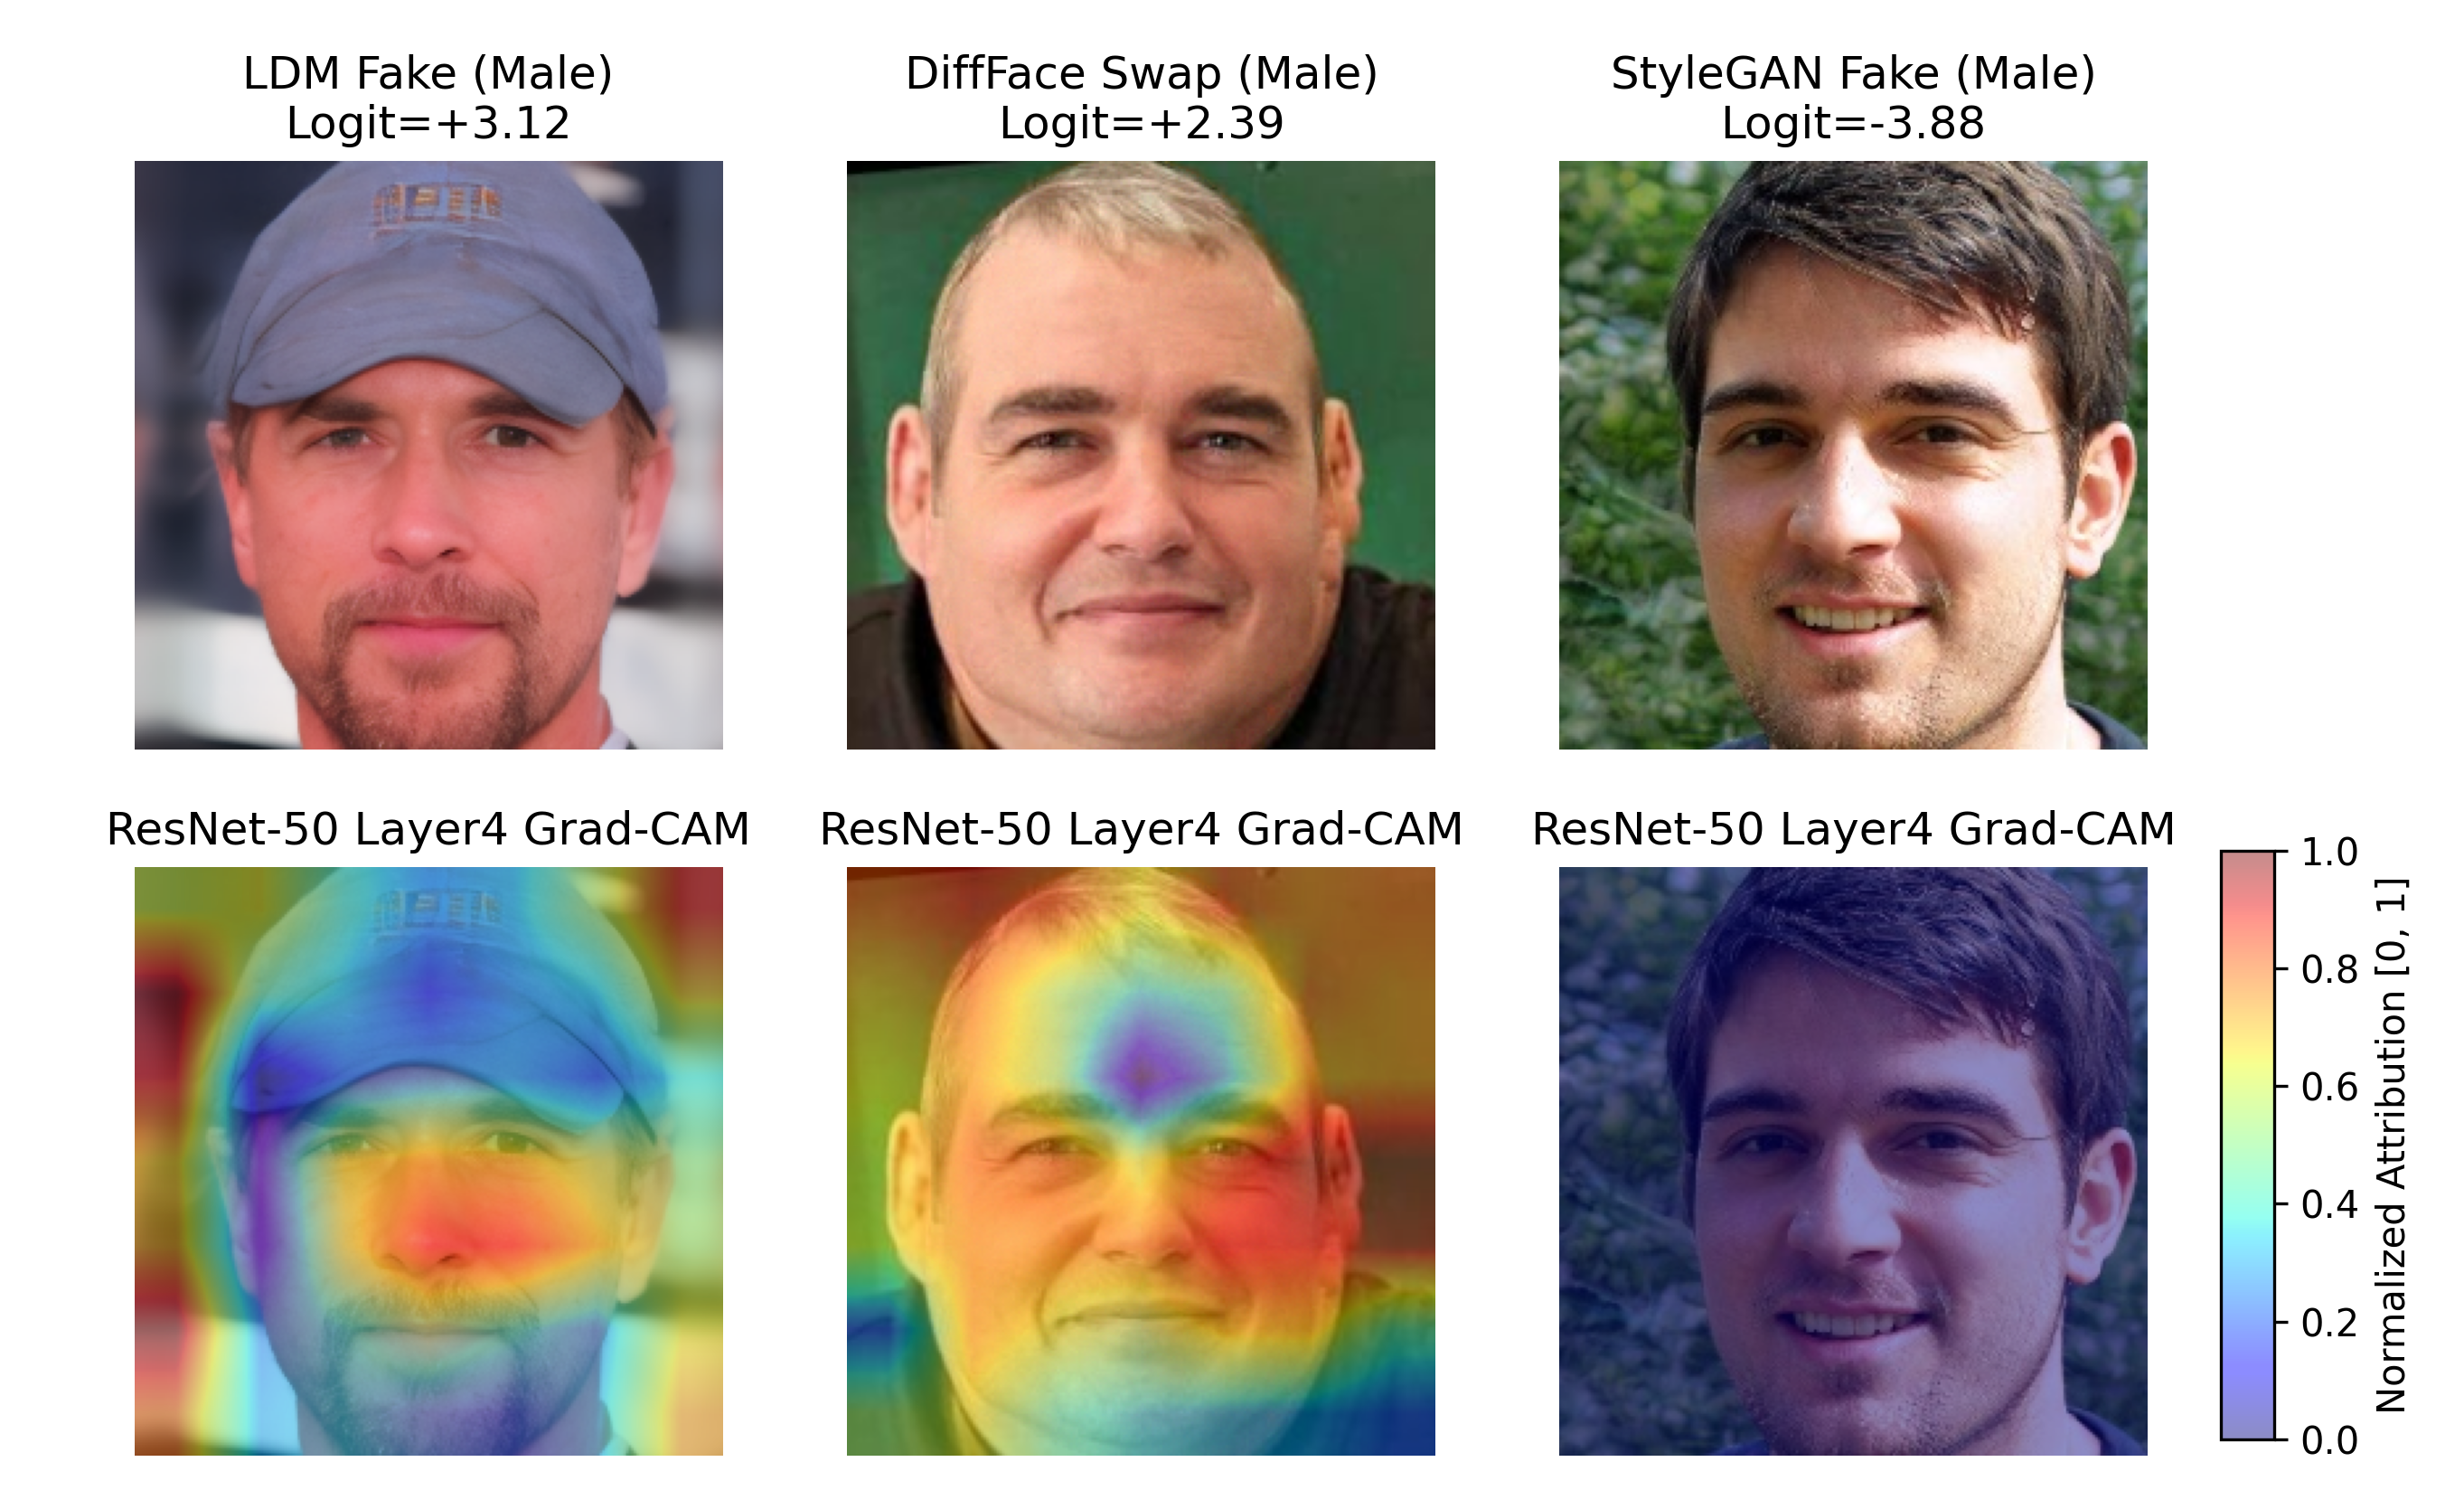
\includegraphics[width=\linewidth]{figures/fig7_gradcam_masking.png}
\caption{ResNet-50 Layer 4 Grad-CAM visualizations across three unseen photorealistic synthetic male face domains (LDM diffusion, DiffFace swap, and StyleGAN) with explicit normalized attribution colorbar $[0,1]$. Correctly detected diffusion and swap samples exhibit strong facial-region attribution ($+3.12$, $+2.39$), whereas the missed StyleGAN sample ($-3.88$) shows negligible activation.}
\label{fig:gradcam}
\end{figure}

\section*{Discussion and Limitations}
Our controlled ablations clarify three foundational lessons for multi-domain deepfake forensics:
\begin{enumerate}
    \item \textbf{Staged Decoupling vs.\ Joint Optimization:} Unfrozen joint training collapsed to $4.5\%$ unseen real recall on LFW ($52.1\%$ accuracy), empirically motivating decoupled specialist representation learning to prevent cross-modal drift.
    \item \textbf{Sample-Dependent Fusion vs.\ Capacity and Two-Way Error Trade-Offs:} Replacing degenerate $T=1$ attention with $L=3$ multi-token \texttt{MHA\_128} and \texttt{GatedFusion} yields verified input-dependent weighting. On untouched \texttt{seen\_test}, fusion trades a slight increase in spatial false positives ($29 \to 35$, authentic recall $99.55\% \to 99.46\%$) for a major reduction in spatial false negatives ($129 \to 75$, synthetic recall $97.92\% \to 98.79\%$) while slashing wavelet false positives by 61.1\% ($90 \to 35$). While capacity-matched MLP, FFN-only, and attention heads converge to statistically indistinguishable in-domain accuracy ($99.10\%$--$99.16\%$, $p_{\text{Holm}}>0.15$), \texttt{MHA\_128} delivers the best strictly PNG-only accuracy ($98.90\%$, $1.04\%$ EER) and lowest unseen calibration error ($\text{ECE}=0.039$, plus significant Brier gains over \texttt{GatedFusion}/\texttt{Fusion\_128}), whereas compact 42K-parameter \texttt{GatedFusion} achieves the highest unseen cross-domain operating accuracy ($85.71\% \pm 0.06\%$, $95.40\%$ DiffFace, $97.7\%$ JPEG $Q=30$) with lowest variance across seeds.
    \item \textbf{Principal Limitations:} First, training solely on diffusion and face-swap generators leaves fine-tuned ResNet-50 vulnerable to completely unseen generative paradigms such as StyleGAN ($0.517$ AUC), where standalone \texttt{Wolter2021\_128} retains stronger ranking ($0.841$ AUC), motivating future integration of frozen foundation encoders (e.g., multi-layer CLIP) alongside wavelet experts. Second, un-hardened dual-stream models remain vulnerable to white-box end-to-end FGSM evasion and unseen additive sensor noise ($\sigma=10$), requiring adversarial training and noise augmentation prior to adversarial deployment. Third, multi-seed variability reflects Phase 2 fusion initializations with fixed Phase 1 experts, and full 439K-image Phase 1 retraining across alternative bottleneck widths ($\{64,128,256\}$) or wavelet decomposition depths ($\{1,2,3,4\}$) was left outside this controlled Phase 2 fusion study (accordingly, no optimality claim over untested widths or depths is made).
\end{enumerate}

\section*{Conclusion}
We presented a decoupled spatial-frequency deepfake detection framework integrating a 128-D RGB ResNet-50 expert (\texttt{Wang2020\_128}) and a 3-level Haar wavelet-packet CNN (\texttt{Wolter2021\_128}) via genuinely sample-dependent multi-token self-attention (\texttt{MHA\_128}) and modality gating (\texttt{GatedFusion}). Evaluated under strict cross-fitted three-way partitioning on 556,082 verified images and four untouched photorealistic unseen domains, cross-fitted two-stream fusion achieves $99.12\%$ held-out accuracy ($0.9997$ AUC, $0.87\%$ EER; trading $+6$ spatial FPs for $-54$ spatial FNs while cutting wavelet FPs by $61.1\%$), leads strictly native PNG-only controls ($98.90\%$, $1.04\%$ EER), decisively defeats unfrozen joint training ($4.5\%$ unseen real recall) and fine-tuned \texttt{Xception} ($43.04\%$ unseen mean), outperforms 12$\times$ larger \texttt{UniversalFakeDetect} on all three unseen diffusion/swap benchmarks, preserves $0.00\%$ demographic FPR disparity on FairFace validation, and reaches up to $95.40\%$ accuracy on unseen DiffFace swaps and $97.7\%$ under severe JPEG $Q=30$ compression.

\section*{Declarations}

\subsection*{Funding}
The authors declare that no funds, grants, or other support were received during the preparation of this manuscript. Open access funding is provided by the Science, Technology \& Innovation Funding Authority (STDF) in cooperation with the Egyptian Knowledge Bank (EKB).

\subsection*{Competing Interests}
The authors declare no competing interests.

\subsection*{Ethical Approval}
Not applicable. All datasets utilized in this study (FairFace, CelebA, FFHQ-256, UTKFace, LFW, StyleGAN 140k, and public Zenodo diffusion repositories) are publicly available academic benchmarks accessed in accordance with their respective research licenses. No human participants were recruited and no new personally identifiable data were collected.

\subsection*{Consent to Participate}
Not applicable. No human participants were involved in this study.

\subsection*{Consent to Publish}
Not applicable. All facial visualizations presented in Figure~\ref{fig:gradcam} depict purely synthetic, AI-generated faces produced by diffusion and GAN models and do not represent real identifiable individuals.

\subsection*{Data Availability}
All datasets analyzed in this study are publicly available through Zenodo (\url{https://doi.org/10.5281/zenodo.10865300} and \url{https://doi.org/10.5281/zenodo.10865065}) and the official public releases of FairFace, CelebA, FFHQ-256, UTKFace, LFW, and 140k Real-and-Fake Faces. Dataset construction manifests, source-by-class contingency tables, and evaluation prediction logs are deposited with the code archive.

\subsection*{Code Availability}
The complete PyTorch source code, capacity-matched ablation heads, cross-fitted evaluation scripts, split manifests, and configuration files are publicly archived on Zenodo (\url{https://doi.org/10.5281/zenodo.21323779})~\cite{ref26} and maintained on GitHub (\url{https://github.com/AbdelrahmanHassan131/Novel-Deepfake-Detection}).

\subsection*{Author Contributions}
Abdelrahman Hassan conceived the study, designed the multi-domain fusion architectures, implemented the training and evaluation codebase, conducted all experiments, and wrote the manuscript. Ahmed Hassan and Hossam Abdelmunim supervised the research, validated the methodological design and statistical analyses, and reviewed and edited the manuscript. All authors read and approved the final manuscript.

\begin{thebibliography}{99}
\bibitem{ref1} Ho, J., Jain, A. \& Abbeel, P. Denoising diffusion probabilistic models. \textit{Advances in Neural Information Processing Systems} \textbf{33}, 6840--6851 (2020).
\bibitem{ref2} Song, J., Meng, C. \& Ermon, S. Denoising diffusion implicit models. In \textit{International Conference on Learning Representations (ICLR)} (2021).
\bibitem{ref3} Dhariwal, P. \& Nichol, A. Diffusion models beat GANs on image synthesis. \textit{Advances in Neural Information Processing Systems} \textbf{34}, 8780--8794 (2021).
\bibitem{ref4} Wang, S.-Y., Wang, O., Zhang, R., Owens, A. \& Efros, A. A. CNN-generated images are surprisingly easy to spot\dots for now. In \textit{Proc.\ IEEE/CVF Conf.\ on Computer Vision and Pattern Recognition (CVPR)}, 8695--8704 (2020).
\bibitem{ref5} Ricker, J., Damm, S., Holz, T. \& Fischer, A. Towards the detection of diffusion model deepfakes. In \textit{Proc.\ 19th Int.\ Joint Conf.\ on Computer Vision, Imaging and Computer Graphics Theory and Applications (VISIGRAPP)}, 447--458 (2024).
\bibitem{ref6} Lin, H., Luo, W., Wei, K. \& Liu, M. Improved Xception with dual attention mechanism and feature fusion for face forgery detection. \textit{IEEE Signal Processing Letters} \textbf{29}, 1639--1643 (2022).
\bibitem{ref7} Yang, S. et al. CrossDF: Improving cross-domain deepfake detection with deep information decomposition. \textit{arXiv preprint arXiv:2310.00359} (2023).
\bibitem{ref8} Wolter, M., Blanke, F., Heese, R. \& Garcke, J. Wavelet-packets for deepfake image analysis and detection. \textit{Machine Learning} \textbf{111}, 4295--4327 (2022).
\bibitem{ref9} Chen, Z. DiffFace - part1 [Data set]. \textit{Zenodo} (2024). \url{https://doi.org/10.5281/zenodo.10865300}.
\bibitem{ref10} Chen, Z. DiffFace - part2 [Data set]. \textit{Zenodo} (2024). \url{https://doi.org/10.5281/zenodo.10865065}.
\bibitem{ref12} R\"{o}ssler, A., Cozzolino, D., Verdoliva, L., Riess, C., Thies, J. \& Nie{\ss}ner, M. FaceForensics++: Learning to detect manipulated facial images. In \textit{Proc.\ IEEE/CVF ICCV}, 1--11 (2019).
\bibitem{ref16} Zhao, W. et al. DiffSwap: High-fidelity and controllable face swapping via 3D-aware masked diffusion. In \textit{Proc.\ IEEE/CVF CVPR}, 8568--8577 (2023).
\bibitem{ref21} Kim, K. et al. DiffFace: Diffusion-based face swapping with facial guidance. \textit{Pattern Recognition} \textbf{163}, 111451 (2025).
\bibitem{ref24} Afchar, D., Nozick, V., Yamagishi, J. \& Echizen, I. MesoNet: A compact facial video forgery detection network. In \textit{IEEE WIFS}, 1--7 (2018).
\bibitem{ref25} Wang, S.-Y. CNNDetection GitHub Repository (2020). \url{https://github.com/PeterWang512/CNNDetection.git}.
\bibitem{ref26} Hassan, A. Novel Deepfake Detection: Spatial-Frequency Retraining and Fusion Framework [Software]. \textit{Zenodo} (2026). \url{https://doi.org/10.5281/zenodo.21323779}.
\bibitem{ref28} Chollet, F. Xception: Deep learning with depthwise separable convolutions. In \textit{Proc.\ IEEE/CVF CVPR}, 1251--1258 (2017).
\bibitem{ref29} Ye, W., He, X. \& Ding, F. Decoupling forgery semantics for generalizable deepfake detection. \textit{arXiv preprint arXiv:2406.09739} (2024).
\bibitem{ref30} Soudy, A. H. et al. Deepfake detection using convolutional vision transformers and convolutional neural networks. \textit{Neural Computing and Applications} \textbf{36}, 19759--19775 (2024).
\bibitem{ref31} Yan, Z., Zhang, Y., Fan, Y. \& Wu, B. UCF: Uncovering common features for generalizable deepfake detection. In \textit{Proc.\ IEEE/CVF ICCV}, 22412--22423 (2023).
\bibitem{ref36} Liu, Z., Luo, P., Wang, X. \& Tang, X. Deep learning face attributes in the wild. In \textit{Proc.\ IEEE ICCV}, 3730--3738 (2015).
\bibitem{ref41} Ojha, U., Li, Y. \& Lee, Y. J. Towards universal fake image detectors that generalize across generative models. In \textit{Proc.\ IEEE/CVF CVPR}, 24480--24489 (2023).
\bibitem{ref42} Chen, B. et al. DRCT: Diffusion reconstruction contrastive training towards universal detection of diffusion generated images. In \textit{Proc.\ ICML} (2024).
\bibitem{ref43} Alkishri, W., Kamal, S. \& Yousif, J. Deepfake detection via frequency-aware Vision Transformer and bidirectional cross-attention fusion with post-processing robustness. \textit{Information} \textbf{17}(9), 819 (2026). \url{https://doi.org/10.3390/info17090819}.
\bibitem{ref44} Pandey, M., Koundal, D. \& Kumar, S. LGF-Net: a spatial-frequency deepfake detection network with learnable Gabor filters and gated cross-modal fusion. \textit{Discover Computing} \textbf{29}, 634 (2026). \url{https://doi.org/10.1007/s10791-026-10548-5}.
\bibitem{ref45} Kashiani, H., Talemi, N. A. \& Afghah, F. FreqDebias: Towards generalizable deepfake detection via consistency-driven frequency debiasing. In \textit{Proc.\ IEEE/CVF CVPR}, 820 (2025). \url{https://doi.org/10.1109/CVPR52734.2025.00820}.
\bibitem{ref46} Karkkainen, K. \& Joo, J. FairFace: Face attribute dataset for balanced race, gender, and age for bias measurement and mitigation. In \textit{Proc.\ IEEE/CVF WACV}, 1548--1558 (2021).
\bibitem{ref47} Karras, T., Laine, S. \& Aila, T. A style-based generator architecture for generative adversarial networks (FFHQ). In \textit{Proc.\ IEEE/CVF CVPR}, 4401--4410 (2019).
\bibitem{ref48} Zhang, Z., Song, Y. \& Qi, H. Age progression/regression by conditional adversarial autoencoder (UTKFace). In \textit{Proc.\ IEEE/CVF CVPR}, 5810--5818 (2017).
\bibitem{ref49} Huang, G. B., Mattar, M., Berg, T. \& Learned-Miller, E. Labeled Faces in the Wild: A database for studying face recognition in unconstrained environments. In \textit{Workshop on Faces in 'Real-Life' Images, ECCV} (2008).
\end{thebibliography}

\clearpage
\section*{Appendix: Statistical Verification, Per-Seed Results, and Reproducibility}

\begin{table}[H]
\centering
\caption{Complete statistical audit on untouched \texttt{seen\_test} ($n=12,729$): identity-cluster bootstrap 95\% confidence intervals (1,000 identity-cluster resamples), all four unrounded per-seed accuracies and EERs (seeds $\{42, 100, 2024, 3407\}$ with fixed Phase 1 experts), two-sided paired $t$-test Cohen's $d$ and Holm--Bonferroni adjusted $p$-values (\texttt{MHA\_128} minus comparator), and the 16-configuration concatenation MLP width/dropout sweep summary.}
\label{tab:stats_appendix}
\resizebox{\linewidth}{!}{%
\begin{tabular}{@{}lcccc@{}}
\toprule
\textbf{Model} & \textbf{Cluster 95\% CI: Acc (\%)} & \textbf{Cluster 95\% CI: AUC} & \textbf{Cluster 95\% CI: EER (\%)} & \textbf{Cluster 95\% CI: Brier} \\
\midrule
\texttt{Wang2020\_128} (RGB) & $[98.41, 99.04]$ & $[0.9993, 0.9997]$ & $[0.85, 1.39]$ & $[0.0107, 0.0147]$ \\
\texttt{Wolter2021\_128} (Freq) & $[97.03, 97.99]$ & $[0.9967, 0.9983]$ & $[1.91, 2.94]$ & $[0.0153, 0.0225]$ \\
\texttt{ConcatMatchedMLP} & $[98.75, 99.36]$ & $[0.9996, 0.9998]$ & $[0.62, 1.12]$ & $[0.0074, 0.0111]$ \\
\texttt{GatedFusion} & $[98.77, 99.35]$ & $[0.9995, 0.9998]$ & $[0.66, 1.14]$ & $[0.0079, 0.0117]$ \\
\textbf{\texttt{MHA\_128} (TokenAttn)} & \textbf{[98.84, 99.38]} & \textbf{[0.9996, 0.9998]} & \textbf{[0.60, 1.05]} & \textbf{[0.0067, 0.0101]} \\
\midrule
\multicolumn{5}{@{}l}{\textit{Four-Seed Unrounded \texttt{seen\_test} Acc / EER (Seeds 42, 100, 2024, 3407) \& Paired Stats vs.\ \texttt{MHA\_128} (Cohen's $d$, $p_{\text{Holm}}$)}} \\
\texttt{MHA\_128} (Reference) & 99.14 / 99.12 / 99.11 / 99.11 & EER: 0.82 / 0.89 / 0.87 / 0.90 & --- & --- \\
vs.\ \texttt{ConcatMatchedMLP} & 99.10 / 99.14 / 99.11 / 99.15 & EER: 0.89 / 0.84 / 0.85 / 0.84 & Acc $d=-0.20$ ($p=1.00$) & Brier $d=-1.57$ ($p=0.258$) \\
vs.\ \texttt{NoAttnFFN} & 99.13 / 99.07 / 99.22 / 99.09 & EER: 0.86 / 0.83 / 0.81 / 0.83 & Acc $d=-0.11$ ($p=1.00$) & Brier $d=+0.13$ ($p=1.00$) \\
vs.\ \texttt{LinearMix} & 99.15 / 99.08 / 99.20 / 99.21 & EER: 0.80 / 0.82 / 0.80 / 0.80 & Acc $d=-0.63$ ($p=0.995$) & Brier $d=+0.71$ ($p=0.995$) \\
vs.\ \texttt{GatedFusion} & 99.10 / 99.10 / 99.10 / 99.10 & EER: 0.92 / 0.90 / 0.92 / 0.92 & Acc $d=+1.19$ ($p=0.318$) & \textbf{Brier $d=-8.69$ ($p=0.0021$)} \\
vs.\ \texttt{Fusion\_128} (Orig) & 99.10 / 99.10 / 99.14 / 99.11 & EER: 0.89 / 0.89 / 0.90 / 0.92 & Acc $d=+0.30$ ($p=1.00$) & \textbf{Brier $d=-4.13$ ($p=0.0186$)} \\
\midrule
\multicolumn{5}{@{}l}{\textit{16-Configuration Concatenation MLP Width/Dropout Sweep ($\text{width}\in\{128,256,384,512\}$, $\text{dropout}\in\{0.1,0.2,0.3,0.5\}$)}} \\
Width 128 (41,729 params) & \texttt{seen\_test} Acc: 99.11--99.15\% & \texttt{seen\_test} AUC: 0.99966--0.99968 & Unseen 4-Dom Acc: 85.25--85.51\% & Unseen AUC: 0.8882--0.9103 \\
Width 256 (99,329 params) & \texttt{seen\_test} Acc: 99.10--99.16\% & \texttt{seen\_test} AUC: 0.99967--0.99969 & Unseen 4-Dom Acc: 85.08--85.28\% & Unseen AUC: 0.8810--0.9130 \\
Width 384 (173,313 params) & \texttt{seen\_test} Acc: 99.10--99.14\% & \texttt{seen\_test} AUC: 0.99967--0.99969 & Unseen 4-Dom Acc: 85.08--85.37\% & Unseen AUC: 0.8969--0.9067 \\
Width 512 (263,681 params) & \texttt{seen\_test} Acc: 99.10--99.12\% & \texttt{seen\_test} AUC: 0.99966--0.99969 & Unseen 4-Dom Acc: 85.08--85.24\% & Unseen AUC: 0.9084--0.9148 \\
\bottomrule
\end{tabular}%
}
\end{table}

All revised experiments were executed on a single NVIDIA L4 GPU (24\,GB VRAM, CUDA 13.0, Python 3.13, PyTorch \texttt{2.14.1+cu130}, \texttt{torchvision}, \texttt{PyWavelets}, \texttt{pytorch-wavelets}, \texttt{scikit-learn}, \texttt{scipy}, \texttt{Pillow}, \texttt{opencv-python}; exact environment pin files and prediction JSON artifacts are archived in the repository). Preprocessing uses direct bilinear resizing of dataset-provided aligned facial crops to $224 \times 224$ with zero external face re-detection. Exact commands for two-expert training and unit-tested evaluation:
{\scriptsize
\begin{verbatim}
git clone --branch GeneralizationDeepFakeDetection \
  https://github.com/AbdelrahmanHassan131/Novel-Deepfake-Detection.git
cd Novel-Deepfake-Detection && pip install -r requirements.txt

# Phase 1: Train Spatial & Frequency Experts (439,222 LOGO images, BS=128, BF16)
python train.py --arch Wang2020_128 --embed_dim 128 --pretrained --optim adamw \
  --lr 2e-4 --weight_decay 1e-2 --rgb_label_smoothing 0.05 --lr_policy cosine \
  --epochs 5 --aug_recipe custom --jpg_prob 0.8 --blur_prob 0.35 \
  --downscale_prob 0.35 --seed 42
python train.py --arch WolterWavelet2021_128 --embed_dim 128 \
  --wavelet_backend gpu --wavelet_type haar --wavelet_level 3 \
  --wavelet_log_mode signed_log1p --optim adam --lr 5e-4 --weight_decay 1e-4 \
  --lr_policy cosine --epochs 5 --seed 42

# Phase 2 & 3: Cross-Fitted Fusion (lr=3e-4, wd=1e-3, BS=256, 25 ep, s=0.05)
python train.py --arch MHA_128 --fusion_type token_attention --embed_dim 128 \
  --num_heads 4 --rgb_model_path <BEST_WANG_E1> \
  --wavelet_model_path <BEST_WAV_E5> --wavelet_backend gpu --optim adamw \
  --lr 3e-4 --weight_decay 1e-3 --batch_size 256 --epochs 25 --seed 42
python -m unittest tests/test_paper1_revision_suite.py -v
\end{verbatim}
}

\end{document}
